\documentclass{beamer}
\usetheme{shadow}
\usepackage[T1]{fontenc}
\usepackage[utf8]{inputenc}
\usepackage[french]{babel}
\usepackage{graphicx,amsmath,calc,transparent,twemojis}
\usepackage[version=4]{mhchem}
\usepackage{tikz}
\usetikzlibrary{shapes.geometric,decorations.pathmorphing,fit}
\usepackage{pdfpages}
\makeatletter
\setbeamertemplate{footline}
{%
  \leavevmode%
  \hbox{\begin{beamercolorbox}[wd=.5\paperwidth,ht=2.5ex,dp=1.125ex,leftskip=.3cm plus1fill,rightskip=.3cm]{author in head/foot}%
    \usebeamerfont{author in head/foot}\insertshortauthor
  \end{beamercolorbox}%
  \begin{beamercolorbox}[wd=.5\paperwidth,ht=2.5ex,dp=1.125ex,leftskip=.3cm,rightskip=.3cm plus1fil]{title in head/foot}%
    \usebeamerfont{title in head/foot}\insertshorttitle\nobreak\hfill\insertframenumber{} / \inserttotalframenumber\usebeamercolor[fg]{page number in head/foot}\usebeamerfont{page number in head/foot}\usebeamertemplate{page number in head/foot}
  \end{beamercolorbox}}%
  \vskip0pt%
}
\graphicspath{{./figs/}}
\AtBeginSection[]{
  \begin{frame}
  \vfill
  \centering
  \begin{beamercolorbox}[sep=8pt,center,shadow=true,rounded=true]{title}
    \usebeamerfont{title}\insertsectionhead\par%
  \end{beamercolorbox}
  \vfill
  \end{frame}
}
\setbeamercovered{dynamic}
\beamertemplatetransparentcovered
\newlength{\@minione}
\newlength{\@minitwo}
\newcommand{\juxt}[3][0.48]{%
\setlength{\@minione}{#1\textwidth}%
\setlength{\@minitwo}{0.96\textwidth - \@minione}%
\begin{minipage}[c][5cm][c]{\@minione}
\raggedright#2
\end{minipage}\hfill
\begin{minipage}[c][5cm][c]{\@minitwo}
\raggedright#3
\end{minipage}%
}
\newlength\p@length
\newcommand{\danger}[1]{%
\begin{tikzpicture}[baseline=(X.center)]
\path[use as bounding box] (-0.4,-0.4) rectangle ++(0.8,0.8);
\node[draw=red,very thick,text=red,regular polygon, regular polygon sides=3,rounded corners, inner sep=1pt,font=\bf] (X) at (0,0) {!};%
\end{tikzpicture}
\setlength{\p@length}{\textwidth}%
\addtolength{\p@length}{-1cm}%
\hfill\parbox{\p@length}{\raggedright#1}}

\newcommand{\includefullheightgraphics}[1]{%
\global\beamer@shrinktrue%
\gdef\beamer@shrinkframebox{%
  \setbox\beamer@framebox=\vbox to 0.96\beamer@frametextheight{%
     \centering%
     \includegraphics[height=0.96\beamer@frametextheight]{#1}%
 }%
}}

%%%%
\newcommand{\Emph}[1]{\textcolor{red}{\textbf{#1}}}
\newcommand{\EMPH}[1]{\textcolor{green!60!black}{\textbf{\textit{#1}}}}
\newcommand{\shadowbox}[1]{\raisebox{0pt}[0pt]{\makebox[0pt][c]{#1}}}
%%%%
\newcommand{\logoFFESSM}{%

\includegraphics[height=5mm]{logoFFESSM}%
}
%%%%
\newcommand{\@ver}[1]{%
\makebox(0,0){\vbox{#1}}%
}
\pgfdeclarelayer{background}
\pgfsetlayers{background,main}
\newcommand{\@list@plon}[3][\relax]{%
\def\@tmp{#1}
\ifx#1\relax%
  \def\@tmp{\null}
\fi
\def\@ttmp{#3}
\ifx#3\relax%
  \def\@ttmp{\null}
\fi
\begin{tikzpicture}[every node/.style={text width=5.3cm}]
\node (one) at (0,0) {#2};
\node[anchor=north west] (two) at (one.south west) {\@tmp};
\node[anchor=north west] (three) at (two.south west) {\@ttmp};
\coordinate (po)  at ([xshift=-5pt,yshift=1pt]one.west);
\coordinate (pt)  at ([yshift=-13pt]po);
\coordinate (pth) at ([yshift=-13pt]pt);
\draw[-stealth] (po) .. controls ++(-2pt,-1pt) .. (one.west);
\ifx#1\relax%
\else
\draw[-stealth] (pt) .. controls ++(-2pt,-1pt) .. ([yshift=-13pt]one.west);
\fi
\ifx#3\relax%
\else
\draw[-stealth] (pth) .. controls ++(-2pt,-1pt) .. ([yshift=-26pt]one.west);
\fi
\begin{pgfonlayer}{background}
\node[fit=(po) (one) (two) (three), fill=cyan, rounded corners=5pt] {};
\end{pgfonlayer}
\end{tikzpicture}
}
%%% width = 5.9cm
\newcommand{\@licence}{%
\@list@plon[Valable du 1~septembre au 31~décembre de l'année suivante]{Responsabilité civile}{\relax}\\\medskip
\rule{1.985cm}{0pt}\frame{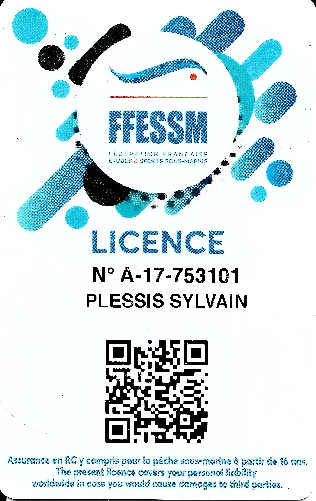
\includegraphics[height=3.752cm]{Licence}}
}
\newcommand{\@carte}{%
\@list@plon[équivalence CMAS au dos]{Preuve du niveau (et donc prérogatives)}{\relax}\\\smallskip
\rule{1.325cm}{0pt}\frame{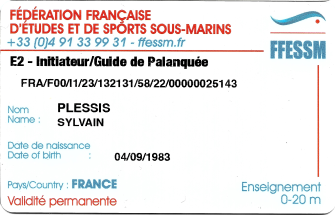
\includegraphics[width=3cm]{carte_niveau_recto}}\\\smallskip
\rule{1.325cm}{0pt}\frame{
\includegraphics[width=3cm]{carte_niveau_verso}}
}
\newcommand{\@CACI}{%
\@list@plon[valable 1 an (accident ou maladie~!)]{Obligatoire}{Préférer un médecin fédéral}\\\smallskip
\rule{1.6295cm}{0pt}\frame{
\includegraphics[height=3.752cm]{CACI}}
}
\newcommand{\@carnet}{%
\@list@plon[Existe sous forme numérique\\\scriptsize\url{https://carnet.ffessm.fr/bienvenue}]{Expérience}{\relax}\\\smallskip
\rule{1.074cm}{0pt}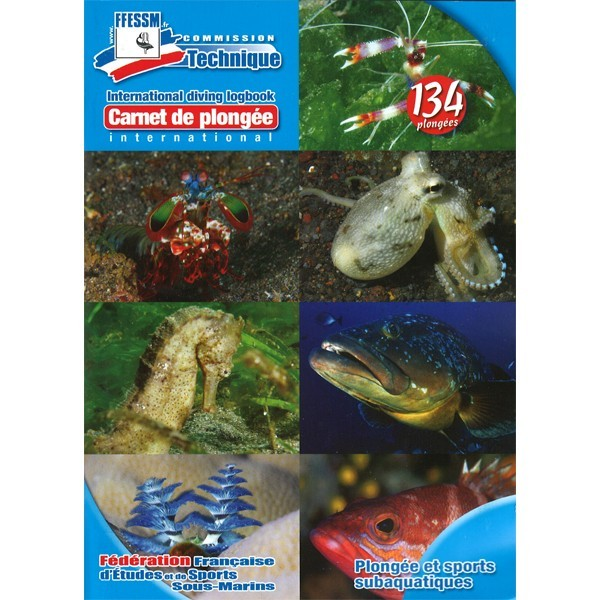
\includegraphics[height=3.752cm]{carnet_plongee}
}
\def\make@over#1{
\expandafter\gdef\csname#1\endcsname##1{\visible<##1>{\@ver{\csname @#1\endcsname}}}
}
\make@over{licence}
\make@over{carte}
\make@over{CACI}
\make@over{carnet}

\newcommand{\photo@text}[1]{%
\transparent{0.5}{\colorbox{white}{\transparent{1}#1}}
}
\newcommand<>{\photo}[3][\relax]{%
\includegraphics#4[width=#3]{#2}%
\ifx#1\relax\else%
  \only#4{\makebox[0pt][c]{\raisebox{5pt}{\photo@text{#1}\rule{#3}{0pt}}}}%
\fi%
}
\newcommand{\zap}[1]{}

\newcommand{\asubsection}[1]{%
\begin{frame}{}
\begin{block}{}
\begin{center}
\large #1
\end{center}
\end{block}
\end{frame}}

\newcommand{\papieren}[1]{%
\makebox[0pt]{
\includegraphics[width=0.6#1]{CACI}}%
\makebox[0pt]{\raisebox{0.4#1}{\rotatebox{-20}{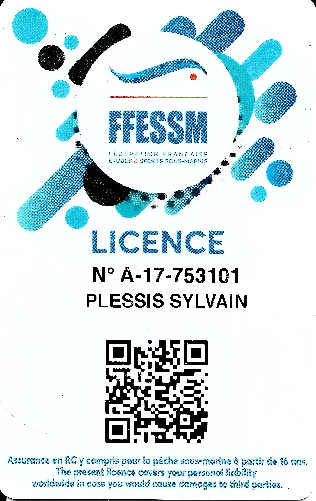
\includegraphics[width=0.2#1]{Licence}}}}%
\makebox[0pt]{\raisebox{0.1#1}{\rotatebox{10}{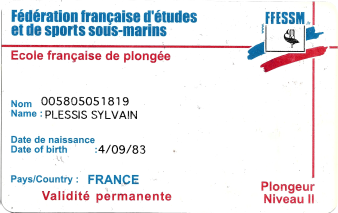
\includegraphics[height=0.2#1]{N2_recto}}}}%
}
\makeatother

\hypersetup{
pdftitle={Théorie N1},
pdfsubject={Cours N1 2024/2025},
pdfauthor={Sylvain Plessis},
pdfkeywords={FFESSM niveau 1}
}
\begin{document}
\setlength{\twemojiDefaultHeight}{15pt}

\title{Théorie N1}
\author[S.~Plessis]{Sylvain Plessis~--~E2}
\newcounter{prevyear}
\setcounter{prevyear}{\the\year}
\addtocounter{prevyear}{-1}
\newcounter{nextyear}
\setcounter{nextyear}{\the\year}
\addtocounter{nextyear}{1}
\date{\theprevyear\ -- \the\year}
\institute{
\includegraphics{logoFFESSM}\hspace{1cm}
\includegraphics[width=1.5cm]{logoAMP}}
\logo{
\includegraphics[width=1cm]{logoAMP}}

\begin{frame}
\addtocounter{framenumber}{-1}
\thispagestyle{empty}
\titlepage
\end{frame}

%%%%%%%%%%%%%%%%%%%
%%%
%%% intro
%%%
%%%%%%%%%%%%%%%%%%
\addtocounter{section}{-1}
\section*{Pourquoi?}
\begin{frame}{Pourquoi faire de la théorie?}
\begin{block}{Une bêbête terrestre sous l'eau}
\og environnement spécifique\fg\ $\Rightarrow$ environnement risqué
\end{block}
\visible<2->{%
\begin{block}{On diminue les risques avec}
\begin{itemize}[<+(1)->]
\item la technologie (matériel),
\item la technique (gestes techniques, attitude).
\end{itemize}
\end{block}
}
\visible<4->{$\Rightarrow$ comprendre, connaître et savoir-faire pour évoluer \EMPH{en toute sécurité.}}
\end{frame}

%%%%%%%%%%%%%%%%%%%
%%%
%%% end intro
%%%
%%%%%%%%%%%%%%%%%%

\begin{frame}
\tableofcontents
\end{frame}

\section{l'Association Montpellier Plongée}
\begin{frame}{L'association}
\begin{itemize}
\item Créée en 1971,
\item \url{https://association-montpellier-plongee.fr/},
\item anciennement club d'IBM, à la piscine du lycée Joffre.
\end{itemize}
\end{frame}

\begin{frame}{L'association}
\begin{block}{piscine}
\begin{itemize}
\item d'octobre à avril, 
\item le mercredi de 19h30 à 21h00.
\end{itemize}
\end{block}
\begin{block}{mer}
\begin{itemize}
\item de mars/avril jusqu'à octobre/novembre,
\item typiquement toutes les deux semaines,
\item deux plongées par jour.
\end{itemize}
\end{block}
\end{frame}

\begin{frame}{Le N1 à l'AMP}
\begin{itemize}
\item Le prix couvre uniquement les sorties techniques en mer
  (la piscine est couverte par l'adhésion),
\item minimum réglementaire 4, au moins 5, c'est mieux!
\end{itemize}

\begin{alertblock}<only@1>{Attention l'agenda}
\danger{ces plongées doivent être faîtes avant le we
  de remise de diplômes!}
\end{alertblock}

\begin{exampleblock}<only@2>{C'est une association}
Uniquement composée de bénévoles! Tout cours/aide/réponse à une question
existentielle est motivé uniquement par le plaisir de partager/faire découvrir.
\end{exampleblock}

\end{frame}


\section{Réglementation}
\begin{frame}{la FFESSM \logoFFESSM}{Fédération Française des Études et Sports Sous-Marins (\url{https://ffessm.fr/})}
\only<1>{\begin{itemize}
\item Fédération nationale;
\item clubs affiliés, Structures Commerciales Agréées (SCA);
\item comprend différents \emph{comités} (nationaux, régionaux, départementaux),
\item conseillés par des \emph{commissions} (\emph{\underline{technique}}, apnée, photographie,\dots),
  aussi aux différents niveaux géographiques.
\end{itemize}}
\includegraphics<2>[width=\textwidth]{ffessm}%
\begin{block}<only@3>{}
La FFESSM définit le cadre de la pratique et l'enseignement en respectant la
loi~--~exception parmi les sports
\end{block}
\centering
\includegraphics<3>[width=2cm]{codeSport}
\end{frame}

\makeatletter
\begin{frame}{Capacités d'un N1}{Ce que vous savez/saurez faire}
\includefullheightgraphics{MFT_competences}
\end{frame}
\makeatother

\begin{frame}{Prérogatives}{Qu'attend-on d'un N1?}
\begin{block}{}
\only<1>{\og Le plongeur niveau 1 (N1) est capable de réaliser des plongées
d’exploration jusqu’à \emph{20~m} de profondeur, au sein d’une \emph{palanquée}, avec
un \emph{guide de palanquée (GP)} qui prend en charge la conduite de la plongée.  Ces
plongées sont réalisées dans le cadre d’une organisation sécurisée, mise en
place par un \emph{directeur de plongée (DP)}, selon les règles définies par le
\textit{Code du Sport} (CdS).\fg}
\only<2->{\begin{itemize}[<+(1)->]
\item Palanquée: 1 à 4 plongeur(s) encadré(s), mêmes profondeur, temps et trajet;
\item en suivant un Guide de Palanquée;
\item Directeur de Plongée: responsable de la sortie et des palanquées.
\end{itemize}}
\end{block}
\end{frame}

\begin{frame}<-7>{Pour plonger}{Un mail typique de l'AMP}
\scriptsize
Listing / pense-bête:\\\medskip
\juxt{%
\begin{itemize}[<+(1)->]
\item \textbf{Licence FFESSM}
\item \textbf{Carte de niveau (sauf formation N1)}
\item \textbf{Certificat médical d’absence de contre-indication en cours de validité (valable 12 mois).}
\item \emph{Carnet de plongée (optionnel)}
\item<6->\color<6->{gray} Bouteille gonflée (sauf si reservé à l'avance)
\item<6->\color<6->{gray} Stab' et détendeurs
\item<6->\color<6->{gray} Ordinateur de plongée, parachute de paliers  (autonomes \& encadrants)
\end{itemize}}
{%
\begin{itemize}[<6->]
\item \color<6->{gray}Combinaison, cagoule, chaussons, gants\dots
\item \color<6->{gray}Masque, palmes, maillot, serviette
\item \color<6->{gray}Plombs (peu disponible sur place) et ceinture ou poches
\item \color<6->{gray}Lampe et appareil photo (optionnel)
\item \color<6->{gray}Vêtements de pluie et/ou protection solaire en fonction de la météo
\item \color<6>{gray}Bouteille d'eau individuelle
\item \color<6->{gray}Repas de midi
\end{itemize}}
\licence{2}\carte{3}\CACI{4}\carnet{5}%
\end{frame}%


\section{Prévention}
\subsection{La pression}
\asubsection{La pression}
\begin{frame}{Barotraumatismes}
\begin{center}\Huge
$\underbrace{\text{baro}}_{\text{pression}}\!\!\underbrace{\text{traumatisme\hspace{2pt}}}_{\text{bobo}}$
\end{center}
\end{frame}

\begin{frame}{Pression et profondeur}
\juxt[0.37]{\includegraphics[height=6cm]{volumePression}}{%
\only<1-6>{\begin{block}{Que se passe-t-il dans l'eau?}
\begin{itemize}[<+->]
\item La pression augmente avec la profondeur\dots
\item \dots\ et écrase tout de plus en plus:
\item[$\Rightarrow$] \emph{les volumes de gaz diminuent.}
\smallskip
\item[] À l'inverse:
\item À la remontée, la pression diminue:
\item[$\Rightarrow$] \emph{les volumes de gaz augmentent.}
\end{itemize}
\end{block}}
\only<7>{\begin{alertblock}{Attention!}
\begin{itemize}
\item Oreilles,
\item masque,
\item poumons,
\item intestins
\item \dots
\end{itemize}
\end{alertblock}}
}
\end{frame}

\begin{frame}{Barotraumatismes}
\centering%
\vspace{6mm}\begin{tikzpicture}[overlay]
\node (pic) at (0,0) {
\includegraphics[width=10cm]{plongeuse}};
\node[above right=3pt,font=\scriptsize] at (pic.south west) {image: Freepik.com};
%%%%% zones
\begin{scope}[every path/.style={fill=red,opacity=0.6}]
%%% sinus
\fill[rotate around={20:(0.1,2.4)}] (0.1,2.4) circle (2pt and 1pt);
\fill[rotate around={-20:(0.5,2.4)}] (0.5,2.4) circle (2pt and 1pt);
%%% oreilles
\fill (-0.12,2.1) circle (1pt and 3pt);
\fill (0.7,2.1) circle (1pt and 3pt);
%%% masque
\fill[opacity=0.3,rounded corners=1pt] (-0.05,2) -- ++(0,0.35) -- ++(0.7,-0.01) -- ++(0,-0.32)  -- ++(-0.2,0) -- ++(-0.1,0.2) -- ++(-0.1,0) -- ++(-0.1,-0.2) -- cycle;
%%% dents
\fill (0.31,1.8) circle (3pt and 1pt);
%%% poumons
\fill (0.1,1.25) circle (3pt and 5pt);
\fill (0.5,1.25) circle (3pt and 5pt);
%%% ventre
\fill (0.3,0.6) circle (5pt);
\end{scope}

\def\xx{-2.5}
\def\start{1.3,3.5}
%%% Masque
\uncover<2-4,20>{\draw<2->[stealth-] (\xx,0.44)node[left]{Masque} -- ++(1,0)  -- (0.1,2.1);}
%%% Ventre
\uncover<5-7,20>{\draw<5->[stealth-] (\xx,-2.4)node[left]{Ventre} -- ++(1,0) -- (0.3,0.6);}
%%% Dents
\uncover<8-10,20>{\draw<8->[stealth-] (\xx,-0.54)node[left]{Dents} -- ++(1,0) -- (0.31,1.8);}
%%% Sinus
\uncover<11-13,20>{\draw<11->[stealth-] (\xx,2.40)  -- (0.1,2.4)  node[pos=0,left]{Sinus};}
\uncover<11-13,20>{\draw<11-> (0.5,2.4) -| ++(0,0.2) -- ([xshift=1cm]\xx,2.40) -- (\xx,2.40);}
%%% Oreilles
\uncover<14-16,20>{\draw<14->[stealth-] (\xx,1.42)node[left]{Oreilles} -- ++(1,0) -- (-0.12,2.1);}
\uncover<14-16,20>{\draw<14-> (0.7,2.1) -| ++(0,0.05) -- ++(-1,0) -- ([xshift=1cm]\xx,1.42) -- (\xx,1.42);}
%%% Poumons
\draw<17->[stealth-] (\xx,-1.52)node[left]{Poumons} -- ++(1,0) -- (0.1,1.25);
\draw<17-> (0.5,1.25) -- ([xshift=1cm]\xx,-1.52) -- (\xx,-1.52);

%%% Masque
\node<2-4> (malert) [below right,font=\tiny] at (\start){%
  \begin{minipage}{95pt}
    \begin{alertblock}{Le masque}
      Effet de succion sur les yeux
    \end{alertblock}
  \end{minipage}
};
\node<3-4> (mblock) [right,below,font=\tiny] at (malert.south) {\begin{minipage}{95pt}\begin{block}{Si ça arrive}Pas grave\end{block}\end{minipage}};
\node<4>            [right,below,font=\tiny] at (mblock.south) {\begin{minipage}{95pt}\begin{exampleblock}{Prévention}Souffler dans le masque par le nez à la descente. Ne pas trop serrer le masque.\end{exampleblock}\end{minipage}};
%%% Ventre
\node<5-7> (valert) [below right,font=\tiny] at (\start){%
  \begin{minipage}{95pt}
    \begin{alertblock}{Du gaz dans les intestins}
      Gaz de digestion $\Rightarrow$ douleurs au ventre à la remontée
    \end{alertblock}
  \end{minipage}
};
\node<6-7> (vblock) [right,below,font=\tiny] at (valert.south) {\begin{minipage}{95pt}\begin{block}{Si ça arrive}Ne pas se retenir.\end{block}\end{minipage}};
\node<7>             [right,below,font=\tiny] at (vblock.south) {\begin{minipage}{95pt}\begin{exampleblock}{Prévention}Pas de choucroute la veille~!\end{exampleblock}\end{minipage}};
%%% Dents
\node<8-10> (dalert) [below right,font=\tiny] at (\start){%
  \begin{minipage}{95pt}
    \begin{alertblock}{Des cavités dans les dents}
      Bulle d'air coincée dans une cavité $\Rightarrow$ douleurs à la remontée, peut endommager la dent.
    \end{alertblock}
  \end{minipage}
};
\node<9-10> (dblock) [right,below,font=\tiny] at (dalert.south) {\begin{minipage}{95pt}\begin{block}{Si ça arrive}Faire sortir la bulle, sinon se préparer à une remontée douloureuse.\end{block}\end{minipage}};
\node<10>             [right,below,font=\tiny] at (dblock.south) {\begin{minipage}{95pt}\begin{exampleblock}{Prévention}Aller chez le dentiste tous les ans~!\end{exampleblock}\end{minipage}};
%%% Sinus
\node<11-13> (salert) [below right,font=\tiny] at (\start)  {%
  \begin{minipage}{95pt}
    \begin{alertblock}{Les sinus bouchés}
      Bulles d'air coincées dans les sinus $\Rightarrow$ douleurs à la remontée et à la descente.
    \end{alertblock}
  \end{minipage}
};
\node<12-13> (sblock) [right,below,font=\tiny] at (salert.south) {\begin{minipage}{95pt}\begin{block}{Si ça arrive}Prévenir le GP tout de suite~! Ne pas forcer~! Pas de médicaments~!\end{block}\end{minipage}};
\node<13>            [right,below,font=\tiny] at (sblock.south) {\begin{minipage}{95pt}\begin{exampleblock}{Prévention}On ne plonge pas enrhumé(e)~!\end{exampleblock}\end{minipage}};
%%% oreilles
\node<14-16> (oalert) [below right,font=\tiny] at (\start) {\begin{minipage}{95pt}\begin{alertblock}{Oreilles bouchées}Oreille(s) non équilibrée(s) à la descente/remontée.\end{alertblock}\end{minipage}};
\node<15-16> (oblock) [right,below,font=\tiny] at (oalert.south) {\begin{minipage}{95pt}\begin{block}{Si ça arrive}Prévenir le GP tout de suite~! On ne force pas~!\end{block}\end{minipage}};
\node<16>            [right,below,font=\tiny] at (oblock.south) {\begin{minipage}{95pt}\begin{exampleblock}{Prévention}On ne plonge pas enrhumé(e)~! On équilibre fréquemment \Emph{uniquement} à la descente.\end{exampleblock}\end{minipage}};
%%% Poumons
\node<17-19> (palert) [below right,font=\tiny] at (\start){%
  \begin{minipage}{95pt}
    \begin{alertblock}{Surpression dans les poumons}
      Accident le plus grave~! Arrive lors d'une remontée en apnée ou sous expiration insuffisante.
    \end{alertblock}
  \end{minipage}
};
\node<18-19> (pblock) [right,below,font=\tiny] at (palert.south) {\begin{minipage}{95pt}\begin{block}{Si ça arrive}Mesures d'urgences.\end{block}\end{minipage}};
\node<19>             [right,below,font=\tiny] at (pblock.south) {%
  \begin{minipage}{95pt}
    \begin{exampleblock}{Prévention}
      \begin{itemize}
        \item \emph{Pas d'apnée} en plongée, 
        \item \Emph{jamais} à la remontée.
        \item Souffler \emph{suffisamment} à la remontée,
        \item remonter de façon \emph{contrôlée} et \emph{lente}.
      \end{itemize}
    \end{exampleblock}
  \end{minipage}
};
%%% résumé
\node<20> [below right,font=\tiny,yshift=2pt] at (\start) {%
  \begin{minipage}{95pt}
    \begin{exampleblock}{Au final}
      \begin{itemize}
        \item Souffler dans le masque par le nez à la descente. Ne pas trop serrer le masque.
        \item Pas de choucroute la veille~!
        \item Aller chez le dentiste tous les ans~!
        \item On ne plonge pas enrhumé(e)~!
        \item On équilibre les oreilles fréquemment \Emph{uniquement} à la descente.
        \item \emph{Pas d'apnée} en plongée,
        \item \Emph{jamais} à la remontée.
        \item Souffler \emph{suffisamment} à la remontée, 
        \item remonter de façon \emph{contrôlée} et \emph{lente}.
      \end{itemize}
    \end{exampleblock}
  \end{minipage}
};
\end{tikzpicture}
\end{frame}


\subsection{La dissolution des gaz}
\asubsection{La dissolution des gaz}
\begin{frame}{La saturation}{Éviter les Accidents De Désaturation (ADD)}
Pendant que l'on est au fond
\begin{itemize}[<+->]
\item on respire de l'air sous pression
\item[$\Rightarrow$] on accumule de l'azote dans le corps.
\item Cet azote s'évacue à la remontée (dégazage).
\end{itemize}
\visible<3>{\begin{center}

\includegraphics[width=4cm]{ouverture-canette-boisson-gazeuse}
\end{center}}
\end{frame}

\begin{frame}{La remontée est maîtrisée}
\begin{block}{}
\begin{itemize}[<+->]
\item Remontée avec son guide de palanquée (moins vite que les plus petites bulles);
\item éventuellement faire des paliers;
\item rester dans des profils de plongée sécuritaires (\emph{c.f.} courbe sans palier obligatoire).
\end{itemize}
\end{block}
\end{frame}

\begin{frame}{Facteurs favorisants}
Attention, ces accidents dépendent:
\begin{itemize}[<+(1)->]
\item de l'individu,
\item de l'état de santé général (obésité, cigarette, \dots), de l'âge (plus de 40 ans),
\item de l'état de forme physique et morale (manque de sommeil, stress, \dots).
\end{itemize}
\end{frame}

\begin{frame}{Signes}
\juxt{%
\begin{itemize}
\item Douleurs, 
\item fourmillements,
\item grande fatigue,
\item maux de tête,
\item vertiges,
\item nausées,
\item vomissements\dots
\end{itemize}
}{%
\begin{alertblock}<2>{}
\danger{En cas de doute on se signale}
\end{alertblock}
}
\end{frame}

\begin{frame}{Courbe de plongée sans palier obligatoire}
\centering\includegraphics[height=6cm]{courbe_secu}
\end{frame}

\zap{ %% »
\begin{frame}{C'est quoi trop profond, c'est combien trop longtemps?}
{1\up{ère} réponse: les tables MN90. Le principe}
\begin{itemize}[<+->]
\item Pour un temps à une profondeur, elles donnent les paliers à respecter,
  sous hypothèse:
  \begin{itemize}
  \item profil carré,
  \item vitesse de remontée entre 15 et 17 m/min.
  \end{itemize}
\item[$\Rightarrow$] La profondeur max donne le temps sans palier et les paliers à respecter
  le cas échéant.
  Les tables donnent aussi l'état de saturation à la fin de la plongée.\\
  $\Rightarrow$ État de saturation au démarrage de la plongée suivante.
\end{itemize}
\end{frame}

\begin{frame}{C'est quoi trop profond, c'est combien trop longtemps?}
{1\up{ère} réponse: les tables MN90. Un exemple}
\begin{itemize}[<+->]
\item Première plongée le matin, 35 min à 20 mètres max, sortie à 11h25.
\item[$\Rightarrow$] Pas de paliers, groupe de saturation E.
\item Deuxième plongée l'après-midi, à 14h15, 40 min à 15 mètres max.
\item[$\Rightarrow$] 2h50 de temps entre les plongées,
\item[$\Rightarrow$] 13 minutes de pénalisation à ajouter,
\item[$\Rightarrow$] 53 minutes à 15 mètres, pas de palier.
\end{itemize}
\end{frame}

\begin{frame}{C'est quoi trop profond, c'est combien trop longtemps?}
{1\up{ère} réponse: les tables MN90. Dans la pratique}
Elles sont peu utilisées, le profil carré n'est pas réaliste, mais il reste
sécuritaire.

Elles nécessitent de se tenir dans le détail aux caractéristiques 
prévues de la plongée, avec peu de capacité d'adaptation, recalculer sous
l'eau n'est pas simple!
\end{frame}

\begin{frame}{C'est quoi trop profond, c'est combien trop longtemps?}
{2\up{nde} réponse: un ordinateur de plongée.}
\only<1>{Plus fin que les tables, prend en compte le profil réel de la plongée
et calcule en temps réel. Permet de comparer le profil réel au profil prévu,
permet d'être adaptable.}
\only<2->{\begin{alertblock}{ATTENTION}
Être adaptable ne signifie pas ne pas respecter les paramètres de
plongée établis par le DP!
\only<3->{%

Un ordinateur n'est pas parole d'évangile, il faut le comprendre pour l'utiliser.
Il faut savoir le paramétrer, savoir sous quels paramètres il est actif, et
\emph{ne pas changer d'ordinateur entre deux plongées successives!}}
\end{alertblock}}
\visible<4>{\centering\large Lire le manuel d'utilisation!}
\end{frame}

\begin{frame}{C'est quoi trop profond, c'est combien trop longtemps?}
{2\up{nde} réponse: un ordinateur de plongée. Quoi ça raconte?}
\begin{minipage}{0.48\textwidth}
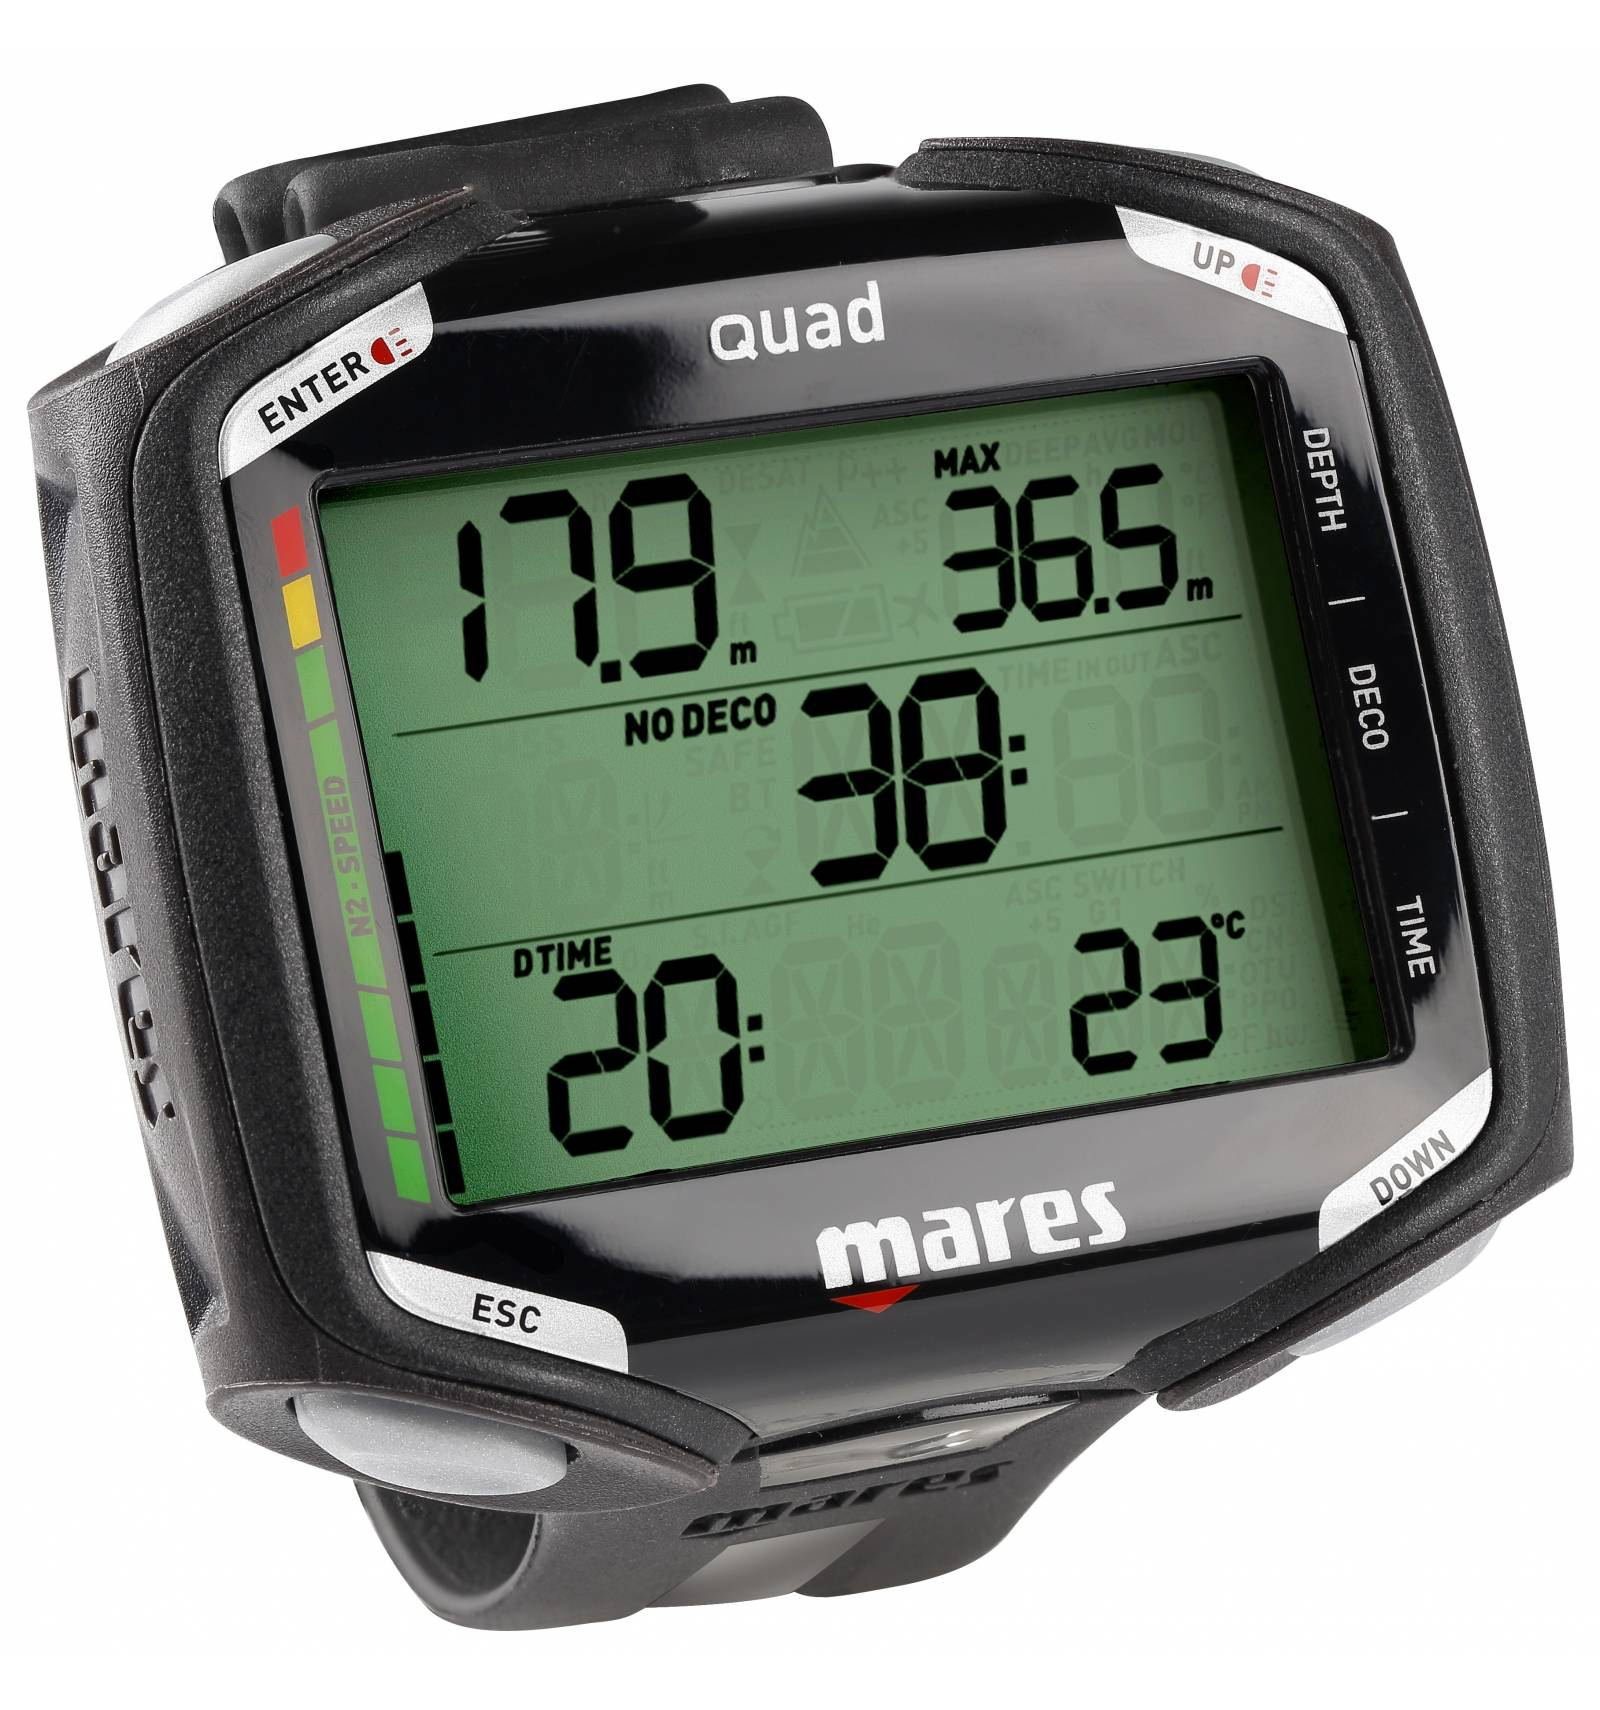
\includegraphics[width=\textwidth]{ordinateur-quad-mares}
\end{minipage}\hfill
\begin{minipage}{0.48\textwidth}
\only<-7>{%
\begin{itemize}[<+->]
\item Profondeur courante,
\item profondeur max,
\item temps de plongée,
\item temps sans palier/paliers à effectuer,
\item mélange utilisé (air, nitrox,\dots),
\item vitesse de remontée,
\item \dots
\end{itemize}}
\only<8>{%
\begin{center}
Il faut lire le manuel de l'ordinateur.
\end{center}
}
\end{minipage}
\end{frame}

} %% end zap «


\subsection{La stabilisation}
\asubsection{La stabilisation}
\begin{frame}{La stabilisation}
{Eurêka!\only<4->{ $\Rightarrow$ Applications}}
\only<-3>{%
\visible<3>{\centering La flottabilité est le bilan de ces deux tendances.}
\juxt{%
\only<2>{Plus on est lourd, plus on coule.}%
\includegraphics<1>[width=\textwidth]{flottabilite}%
\includegraphics<3>[width=\textwidth]{flottabilite3}%
}{%
\only<1>{Plus on est volumineux, plus on flotte}%
\includegraphics<2>[width=\textwidth]{flottabilite2}%
\includegraphics<3>[width=\textwidth]{flottabilite4}%
}}%
\only<4-7>{%
\juxt{%
\begin{itemize}[<+(3)->]
\item La combinaison ajoute du volume
\item[$\Rightarrow$] il faut des plombs pour la compenser.
\end{itemize}%
}{%
\begin{itemize}[<+(3)->]
\item À la descente, la combinaison s'écrase sous l'effet de
  la pression
\item[$\Rightarrow$] il faut gonfler son gilet pour compenser.
\end{itemize}%
}}%
\only<8->{%
\juxt[0.3]{%
\includegraphics[width=0.8\textwidth]{test_flotta}
}{%
\begin{exampleblock}{Test de lestage}
En surface, poumons et gilet vides, l'eau est au niveau
du masque.\\
\alert{On ne coule pas!}\\
\uncover<9>{Se confirme et s'évalue en fin de plongée:\\%
$\left.\begin{array}{l}
\text{50~bars}    \\
\text{3~m}        \\
\text{gilet vide} \\
\end{array}\right\}\Rightarrow$ flottabilité neutre}
\end{exampleblock}
}}
\end{frame}


\subsection{L'essouflement}
\asubsection{L'essouflement}
\begin{frame}{L'essouflement}
{La plongée: un sport tranquille}
\juxt[0.3]{%
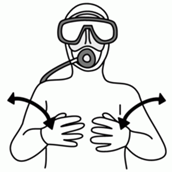
\includegraphics[width=\textwidth]{essouflement}
}{%
\begin{alertblock}<only@-5>{}
\begin{itemize}[<+->]
\item causé par l'excès de \ce{CO2},
\item trop d'efforts physique,
\begin{itemize}
  \item courant,
  \item palmage inefficace,\dots
\end{itemize}
\end{itemize}
\end{alertblock}
\begin{block}<only@-5 | visible@5>{}
\danger{La consommation d'air!\\
Attention à la panne d'air.}
\end{block}%
\begin{exampleblock}<only@6->{}
\begin{itemize}[<+(1)->]
\item On arrête tout effort, on se calme rapidement, 
\item on souffle!
\item On se signale au guide.
\item Vérifier sa consommation.
\end{itemize}
\end{exampleblock}%
}
\end{frame}



\subsection{La température}
\asubsection{La température}
\begin{frame}{Le froid}
\only<-4>{\juxt[0.65]{%
\centering%
\vspace{1cm}%
\newcommand{\circulation}{%
\draw (-1.5,1) arc(90:30:2mm);
\draw (-1.515,1.04) -- ++(45:2mm);
\draw (-1.53,1.08) arc(-30:30:2mm);
\draw (-0.08,1.11) arc(-30:30:2mm);
\draw (-0.08,1.1) --++(20:2mm);
\draw (-0.08,1.09) arc(30:-30:2mm);
\draw (-1.39,1.28) arc(0:90:2mm);
\draw (0.42,1.22) arc(0:60:2mm);
\draw (0.45,1.19) --++(40:2mm);
\draw (0.47,1.16) arc(120:60:2mm);
\draw (1.35,0.4) arc(-90:-150:2mm);
\draw (1.375,0.36) --++(-150:2mm);
\draw (1.4,0.32) arc(130:190:2mm);
\draw (1.28,1.35) arc(180:90:2mm);
\draw[opacity=1,line width=0.4pt] (circ) -- ++(1,0) node[pos=1,right,font=\small]{Circulation};
}
\newcommand{\conduction}{%
\draw (-1.1,1.8) -- ++(45:3mm);
\draw (-1.3,1.9) -- ++(80:3mm);
\draw (-1.5,1.8) -- ++(120:3mm);
\draw (-1.7,0) -- ++(180:3mm);
\draw (-1.5,-0.5) -- ++(180:3mm);
\draw (-0.78,-0.2) -- ++(0:3mm);
\draw (-0.5,1.1) -- ++(90:3mm);
\draw (1.28,1.8) -- ++(45:3mm);
\draw (1.15,1.95) -- ++(100:3mm);
\draw (1,1.9) -- ++(120:3mm);
\draw (0.8,0) -- ++(180:3mm);
\draw (0.8,-0.5) -- ++(180:3mm);
\draw (1.45,-1.05) -- ++(45:3mm);
\draw (2,0.7) -- ++(0:3mm);
\draw[opacity=1,line width=0.4pt] (cond) -- ++(1,0) node[pos=1,right]{Conduction};
}
\begin{tikzpicture}[overlay,yshift=3mm]
\node (pic) at (0,0) {
\includegraphics[height=6.5cm]{plongeurs}};
\node[above left=1pt,font=\footnotesize] at (pic.south east) {image: Freepik.com};
\coordinate (circ) at (-3.4,3);
\coordinate (cond) at (-0.2,3);
\coordinate (vent) at (-3.4,2.6);
\temporal<2>{}{%
\begin{scope}[every path/.style={-stealth,thin,blue}]
\circulation
\end{scope}%
}{%
\begin{scope}[every path/.style={-stealth,thin,blue,opacity=0.4}]
\circulation
\end{scope}%
}
\temporal<3>{}{%
\begin{scope}[every path/.style={-stealth,thin,red,decorate,decoration={snake,amplitude=1pt,segment length=3pt, post=lineto, post length=3pt}}]
\conduction
\end{scope}}{%
\begin{scope}[every path/.style={-stealth,thin,red,decorate,decoration={snake,amplitude=1pt,segment length=3pt, post=lineto, post length=3pt},opacity=0.4}]
\conduction
\end{scope}
}
\visible<4>{\begin{scope}[every path/.style={-stealth,thin,yellow,dashed,dash pattern=on 2pt off 1pt}]
\draw (-1.2,1.35) .. controls ++(-0.1,-0.1) .. (-1.3,1);
\draw (-1.2,1.35) .. controls ++(-0.1,-0.1) .. (-1.1,1);
\draw[solid] (-1.2,1.35) .. controls ++(0.3,0.1) .. (-0.8,1.7);
\draw (1.05,1.45) .. controls ++(0.1,-0.1) .. (1.2,1);
\draw (1.05,1.45) .. controls ++(0.1,-0.1) .. (0.85,1);
\draw[solid] (1.05,1.45) .. controls ++(0.2,0) .. (1.35,1.7);
\draw[line width=0.4pt] (vent) -- ++(1,0) node[pos=1,right]{Ventilation};
\end{scope}}
\end{tikzpicture}%
}
{%
\begin{itemize}[<+(1)->]
\item Combinaison bien ajustée. Humide v/s semi-étanche v/s étanche.
\item Épaisseur de la combinaison, souris, cagoule, gants, chaussons néoprène, \dots
\item Pas grand chose à faire\dots
\end{itemize}
}}
\only<5->{%
\juxt[0.4]{\includegraphics[width=\textwidth]{froid}}{%
Refroidissement du corps environ 25 fois plus vite dans l'eau que dans l'air!
\begin{itemize}[<+(5)->]
\item Augmente la consommation,
\item favorise un essouflement.
\end{itemize}
\begin{alertblock}<+(5)>{}
On n'attend pas d'être en hypothermie pour le signaler! Anticiper
le temps de retour et remontée!
\end{alertblock}}}
\end{frame} 


\subsection{La narcose}
\asubsection{La narcose}
\begin{frame}{La narcose (a.k.a. l'ivresse des profondeurs)}
\begin{block}{Bourré(e) sous l'eau}
\begin{itemize}[<+->]
\item Excès d'azote (\ce{N2}) dans le corps, mêmes effets
  que l'alcool;
\item apparaît rarement avant 30, 35 mètres;
\item[$\Rightarrow$] N1 peu concerné(e)s.
\end{itemize}
\end{block}
\begin{exampleblock}<+->{Si ça arrive}
\begin{itemize}[<+->]
\item Prévenir le GP si on a un doute,
\item il vous prendra en charge, effets temporaires.
\end{itemize}
\end{exampleblock}
\end{frame}


\section{Déroulement d'une sortie plongée à l'AMP}
\subsection{Toute plongée}
\begin{frame}{Avant la plongée}
\centering%
%\includegraphics<1>[width=2cm]{Sorties_2024-2025}%
\includegraphics<1>[width=2cm]{Agenda_AMP}%
\begin{block}<only@1>{}
\begin{itemize}
\item Vérification du niveau pour la plongée;
\item inscription sur le site;
\item pré-paiement suivant la plongée.
\end{itemize}
\end{block}%
\includegraphics<1>[width=2cm]{inscription2}%
%\includegraphics<2>[width=\textwidth]{Sorties_2024-2025}%
\includegraphics<2>[height=6.5cm]{Agenda_AMP}%
\only<3>{\juxt[0.3]{\includegraphics[width=\textwidth]{equipement}}{%
\begin{block}{Préparation du sac}
\begin{itemize}
\item Maillot, serviette, moyens de paiement, crème solaire, vêtements de rechange\dots;
\item équipement: combinaison, masque, détendeur, gilet, palmes, bouteille;
\item paperasse: \Emph{licence}, \Emph{certificat médical}, \Emph{carte niveau}, carnet de plongée;
\item de quoi manger (sandwich/salade/\dots, eau).
\end{itemize}
\end{block}}}%
\includegraphics<4>[width=3cm]{covoit}%
\begin{block}<only@4>{Covoiturage}
Lieu de rendez-vous, prévoir une place dans une voiture ou
proposer des places dans sa voiture
\end{block}%
\end{frame}

\begin{frame}{Sur le lieu de la plongée}
\juxt[0.7]{%
\begin{block}{Papiers!}
Présenter ses papiers au DP
\end{block}
\begin{block}{Préparer ses affaires}
\begin{itemize}
\item Vérification et gréage de son bloc.
\item Bouteille fermée et allongée ou accrochée sur le bateau.
\end{itemize}
\end{block}
\begin{block}{Embarquer}
\begin{itemize}
\item Bloc et affaires fixés sur le bateau, rien ne traine.
\item Combinaison suivant DP/GP.
\end{itemize}
\end{block}}{%
\null\hfill\papieren{\textwidth}\hfill\null\\
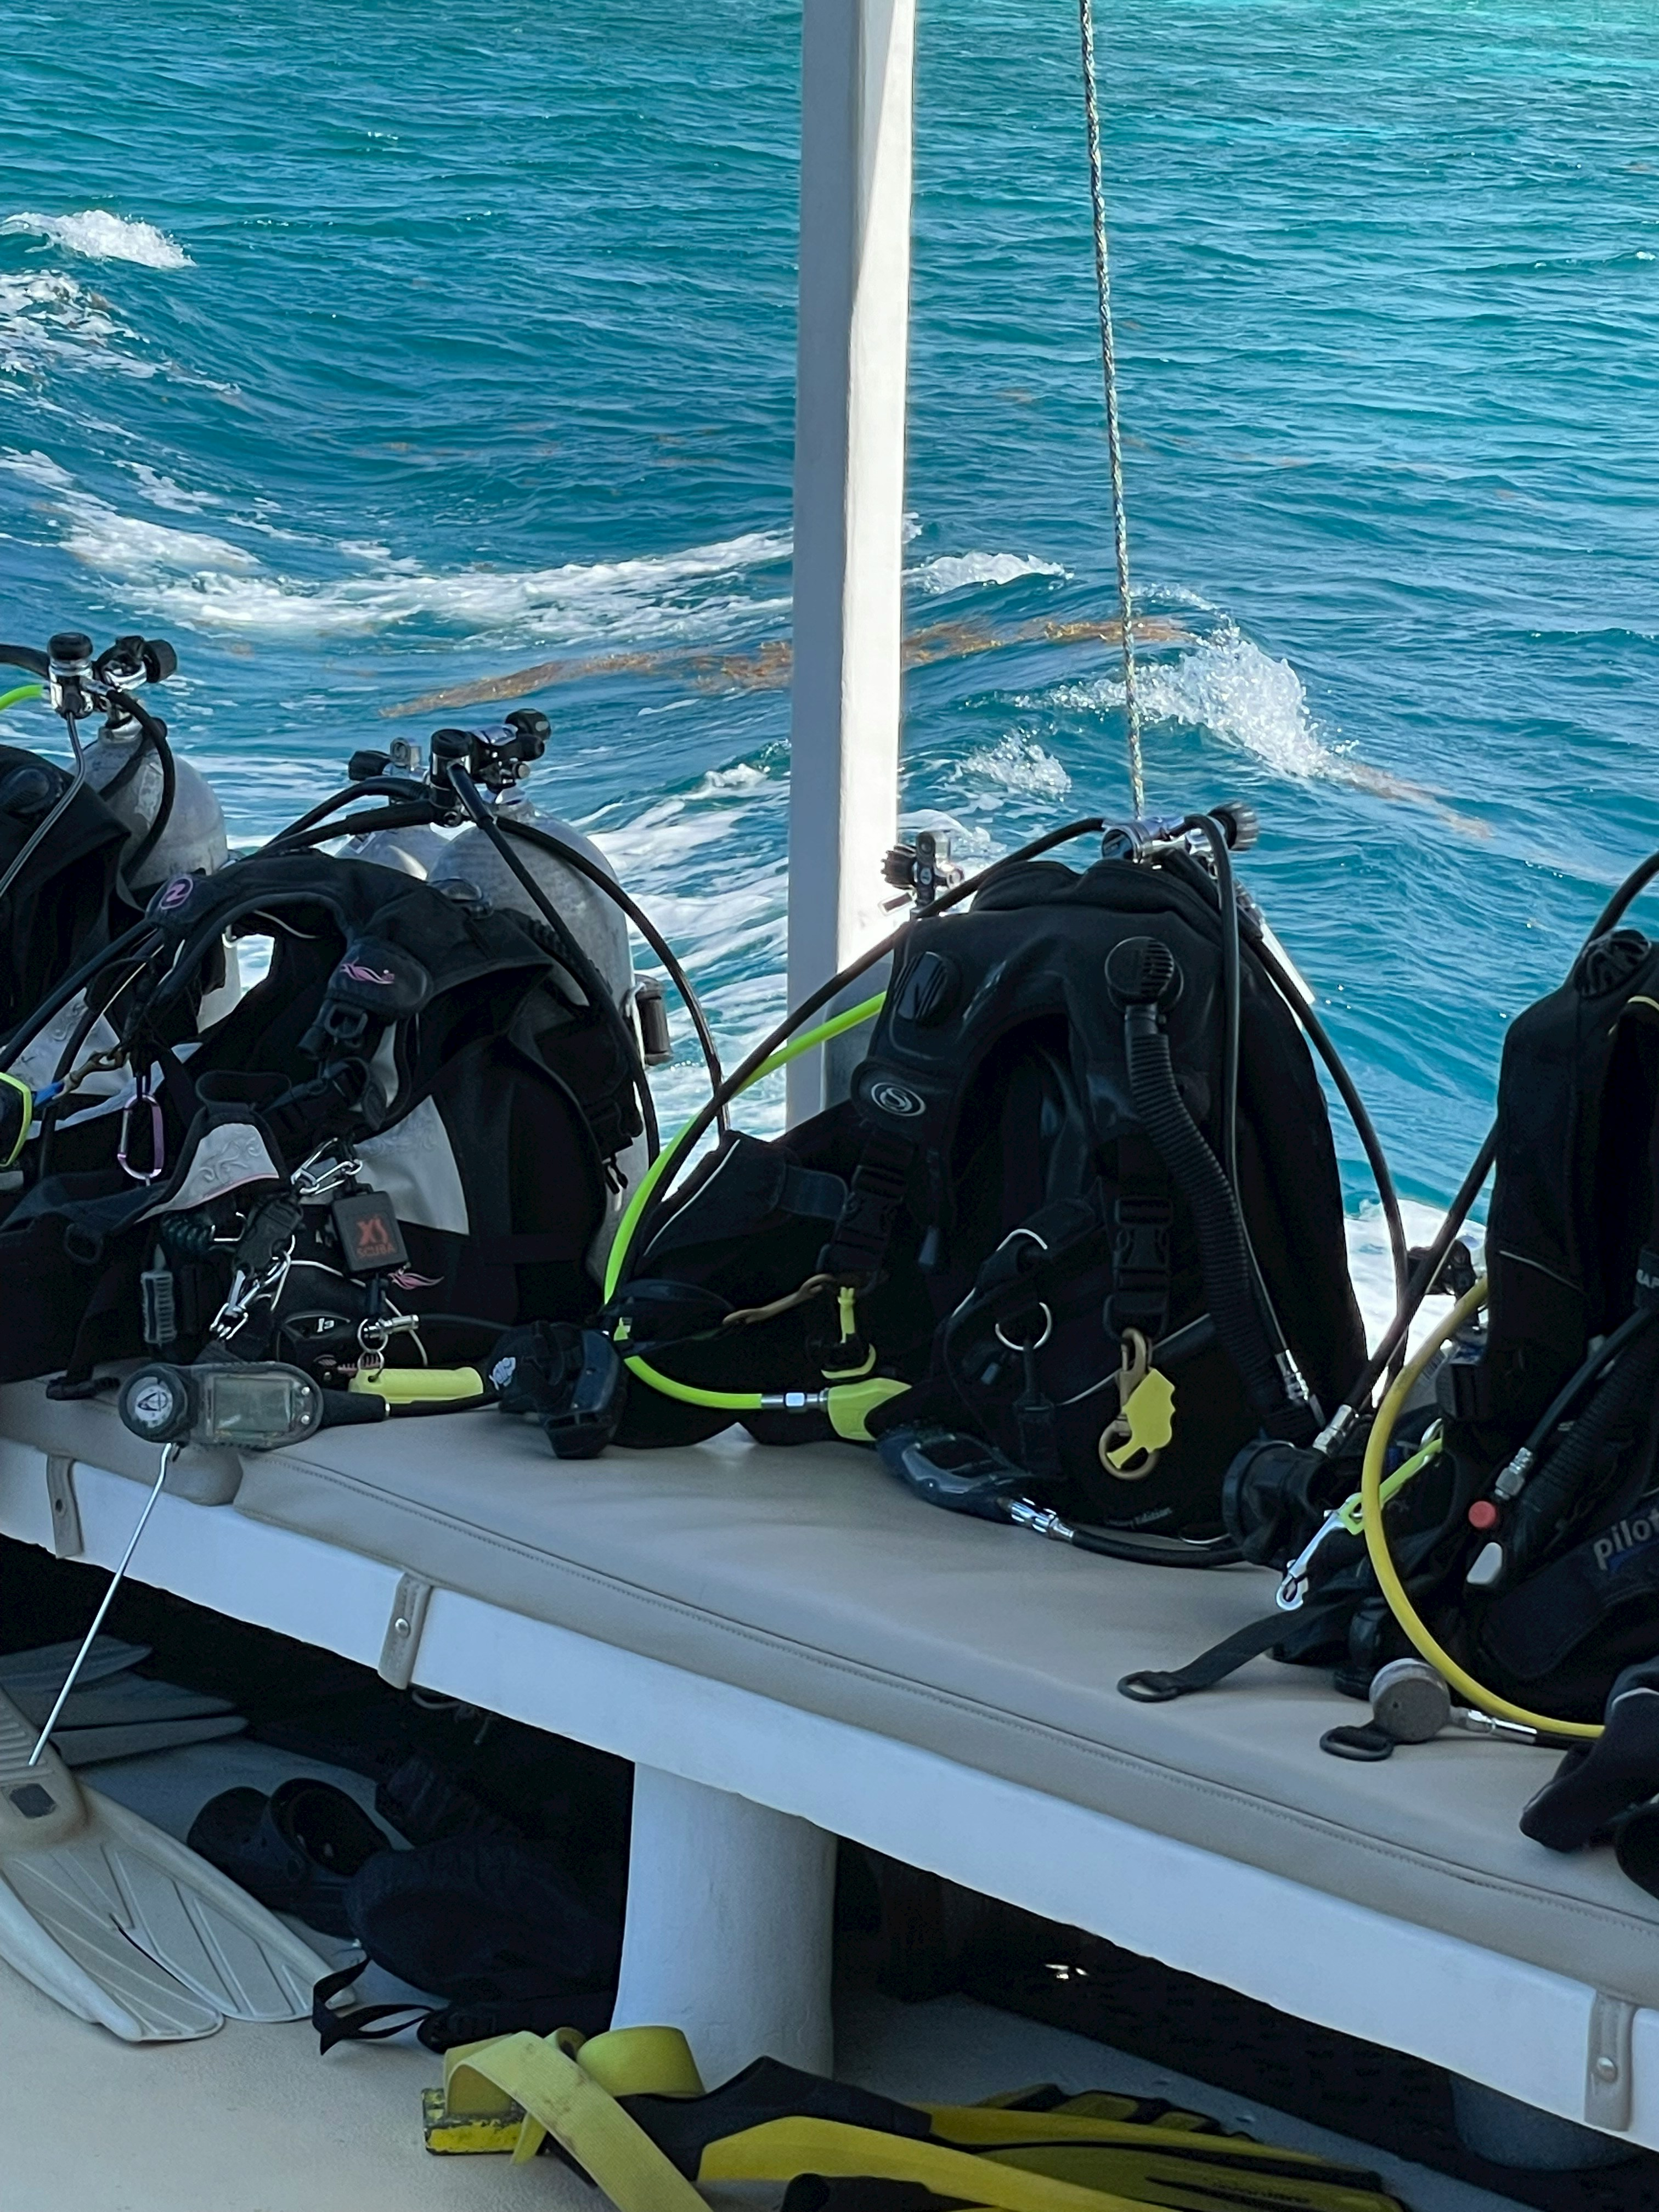
\includegraphics[width=\textwidth]{blocs}
}
\end{frame}

\begin{frame}{Sur le trajet en mer}
\juxt{%
\begin{block}{}
\begin{itemize}[<+->]
\item On ne gêne pas;
\item on écoute les consignes (pilote, directeur de plongée, son guide);
\item on s'équipe (consignes guide);
\item mise à l'eau (bascule arrière, saut droit) \Emph{après} son guide.
\end{itemize}
\end{block}}
{%
\includegraphics<1-2>[width=\textwidth]{bateau}%
\includegraphics<3>[width=\textwidth]{sequipe}%
\includegraphics<4>[width=\textwidth]{saut_droit}%
}
\end{frame}

\begin{frame}{Dans l'eau}
\only<1-3>{\null\hfill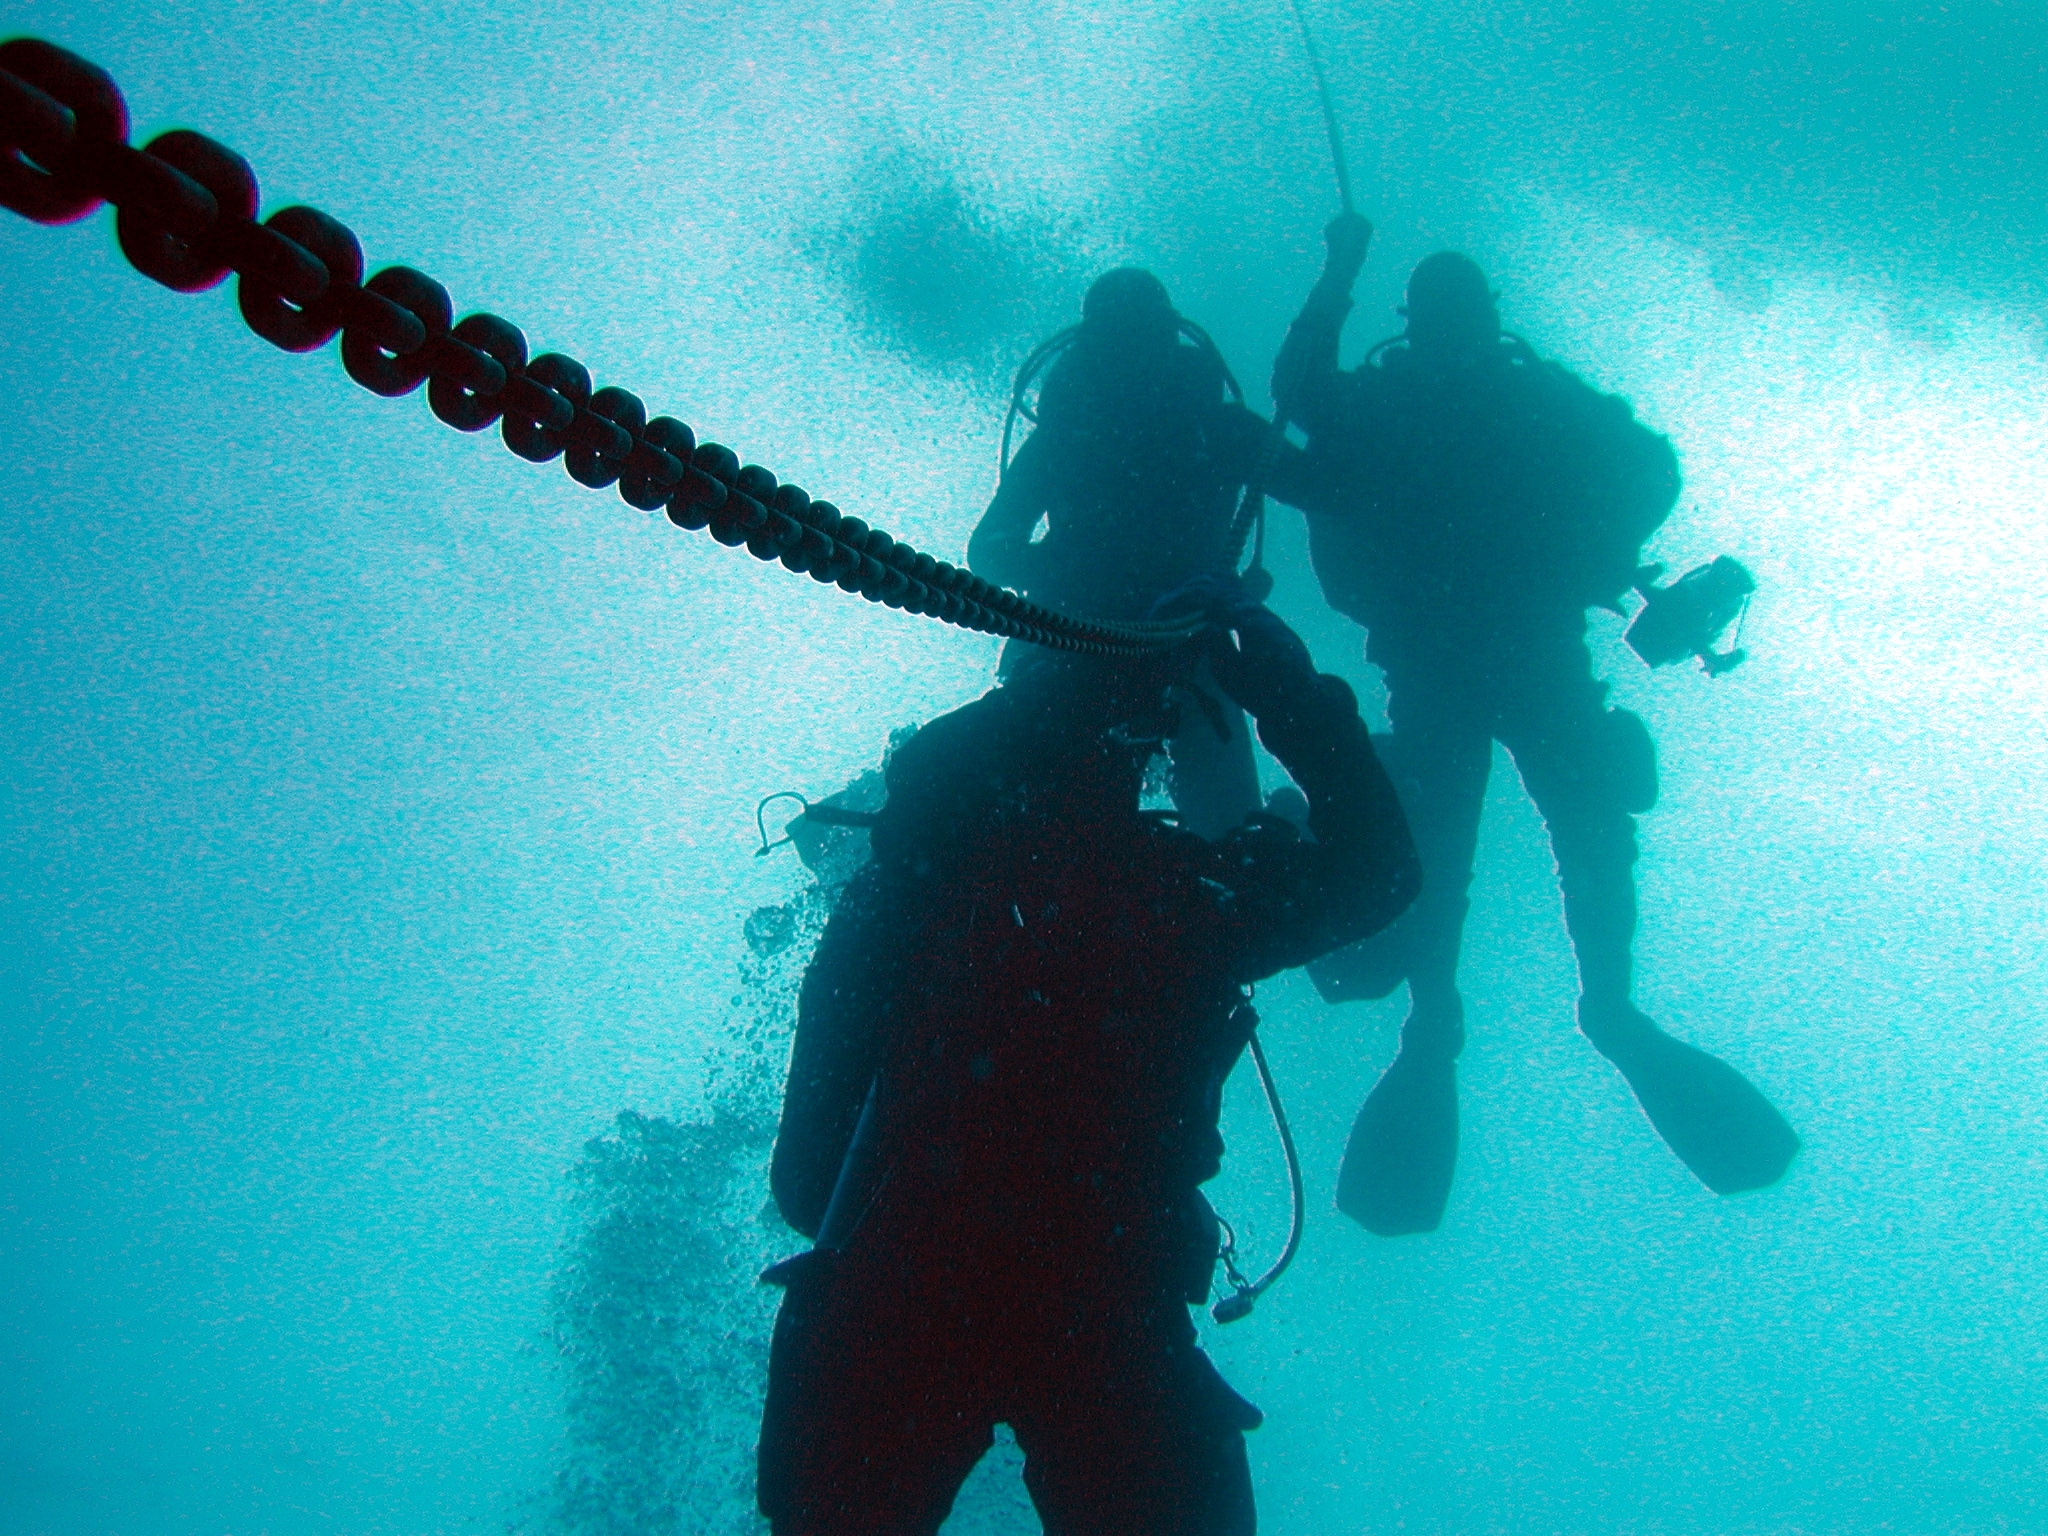
\includegraphics[width=4cm]{descente}\hfill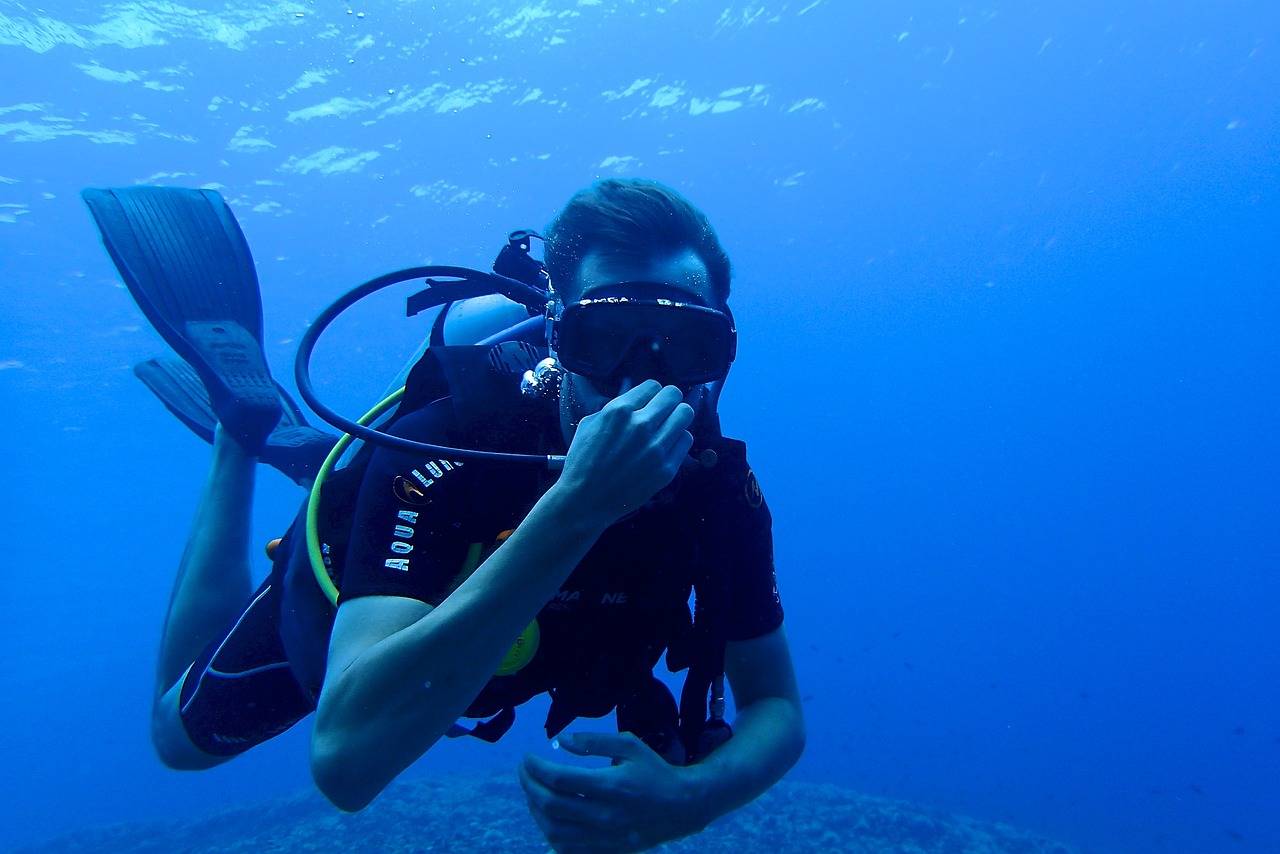
\includegraphics[width=4cm]{oreilles}\hfill\null}%
\begin{block}<only@1-3>{L'immersion}
\begin{itemize}[<+->]
\item Sur signe du guide, phoque ou canard;
\item descente au-dessus du guide;
\item attention aux \Emph{oreilles}, équilibrage tout le long.
\end{itemize}
\end{block}%
\only<4-9>{%
\juxt[0.6]{\begin{block}{La balade}
\begin{itemize}[<+->]
\item Proche du guide, même profondeur;
\item suis ses instructions;
\item on communique, on donne sa consommation d'air;
\item on communique, si froid, si essouflement, si quoi que ce soit;
\item on profite.
\item<+-| alert@+> Si on perd sa palanquée
\end{itemize}
\end{block}}{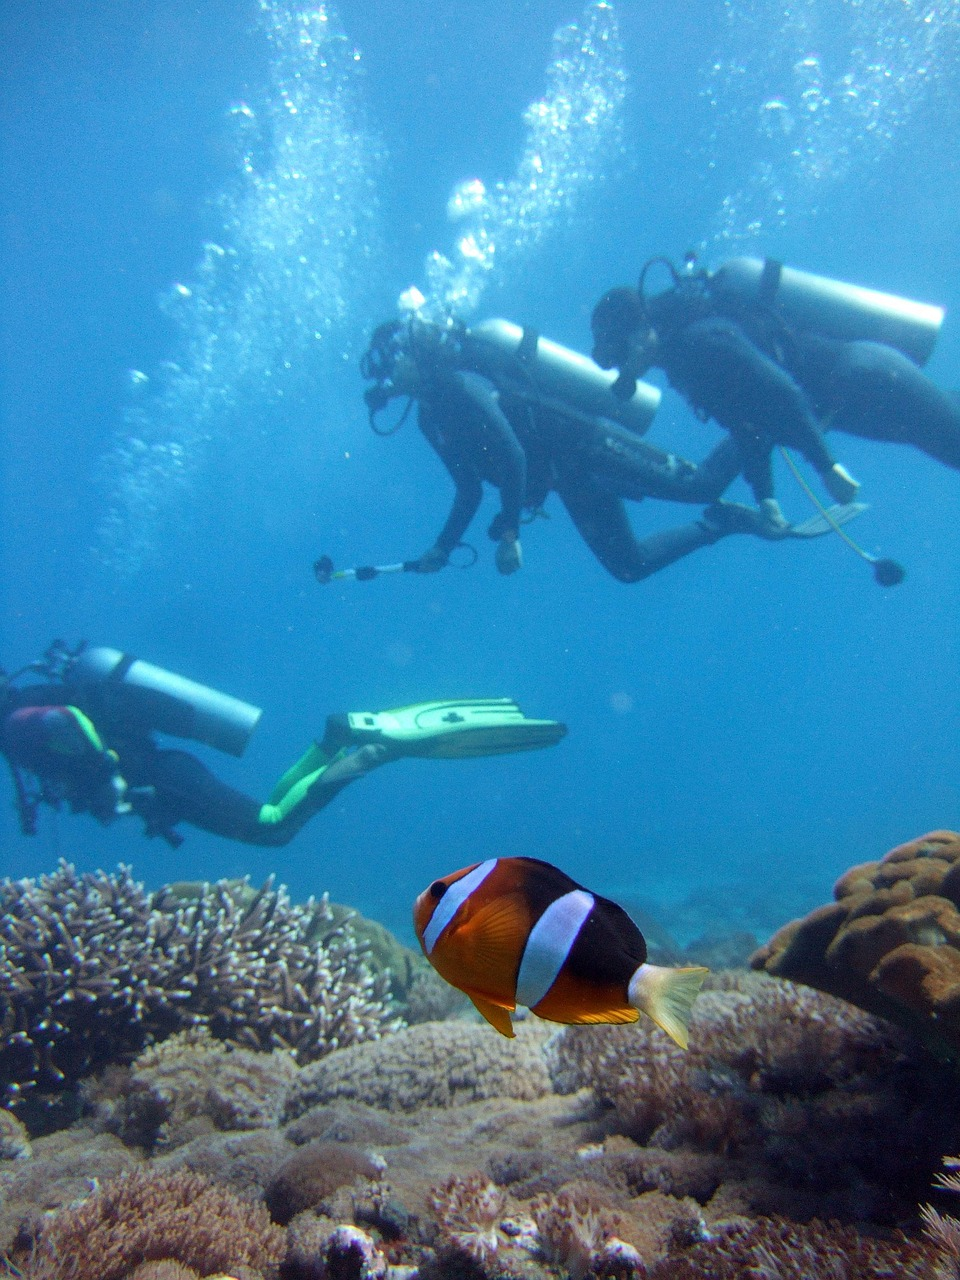
\includegraphics[width=\textwidth]{palanquee}}}
\only<10>{\null\hfill\includegraphics[width=3cm]{recherche}\hfill
\includegraphics[width=3cm]{remontee}\hfill\null}%
\begin{block}<only@10>{}
\begin{itemize}
\item On cherche environ 1~minute, on remonte de quelques
  mètres, on cherche les bulles,
\item on remonte \EMPH{doucement}, en \EMPH{soufflant}, et on se retrouve à la
  surface.
\end{itemize}
\end{block}%
\begin{block}<only@11->{La remontée}
\begin{itemize}[<+(7)->]
\item Sur signe du guide;
\item juste sous le guide;
\item gestion du gilet;
\item on souffle;
\item on n'équilibre pas ses oreilles;
\item palier à 3 mètres possible;
\item tour d'horizon à l'approche de la surface;
\item gonfle le gilet à la surface;
\item remontée sur le bateau sur indication du guide,
  masque sur le visage et détendeur en bouche. On ne traîne pas sous l'échelle.%
\end{itemize}%
\end{block}%
\only<11->{%
\vskip -1cm\makebox[0pt][l]{\raisebox{1.8cm}[0pt][0pt]{\rule{0.6\textwidth}{0pt}%
\includegraphics<11-12>[width=4cm]{up}%
\includegraphics<13>[width=3cm]{gilet}%
\includegraphics<14-17>[width=4cm]{souffle}%
\includegraphics<18>[width=4cm]{surface}%
\includegraphics<19>[width=4cm]{echelle}%
}}}%
\end{frame}

\begin{frame}{Le retour}
\null\hfill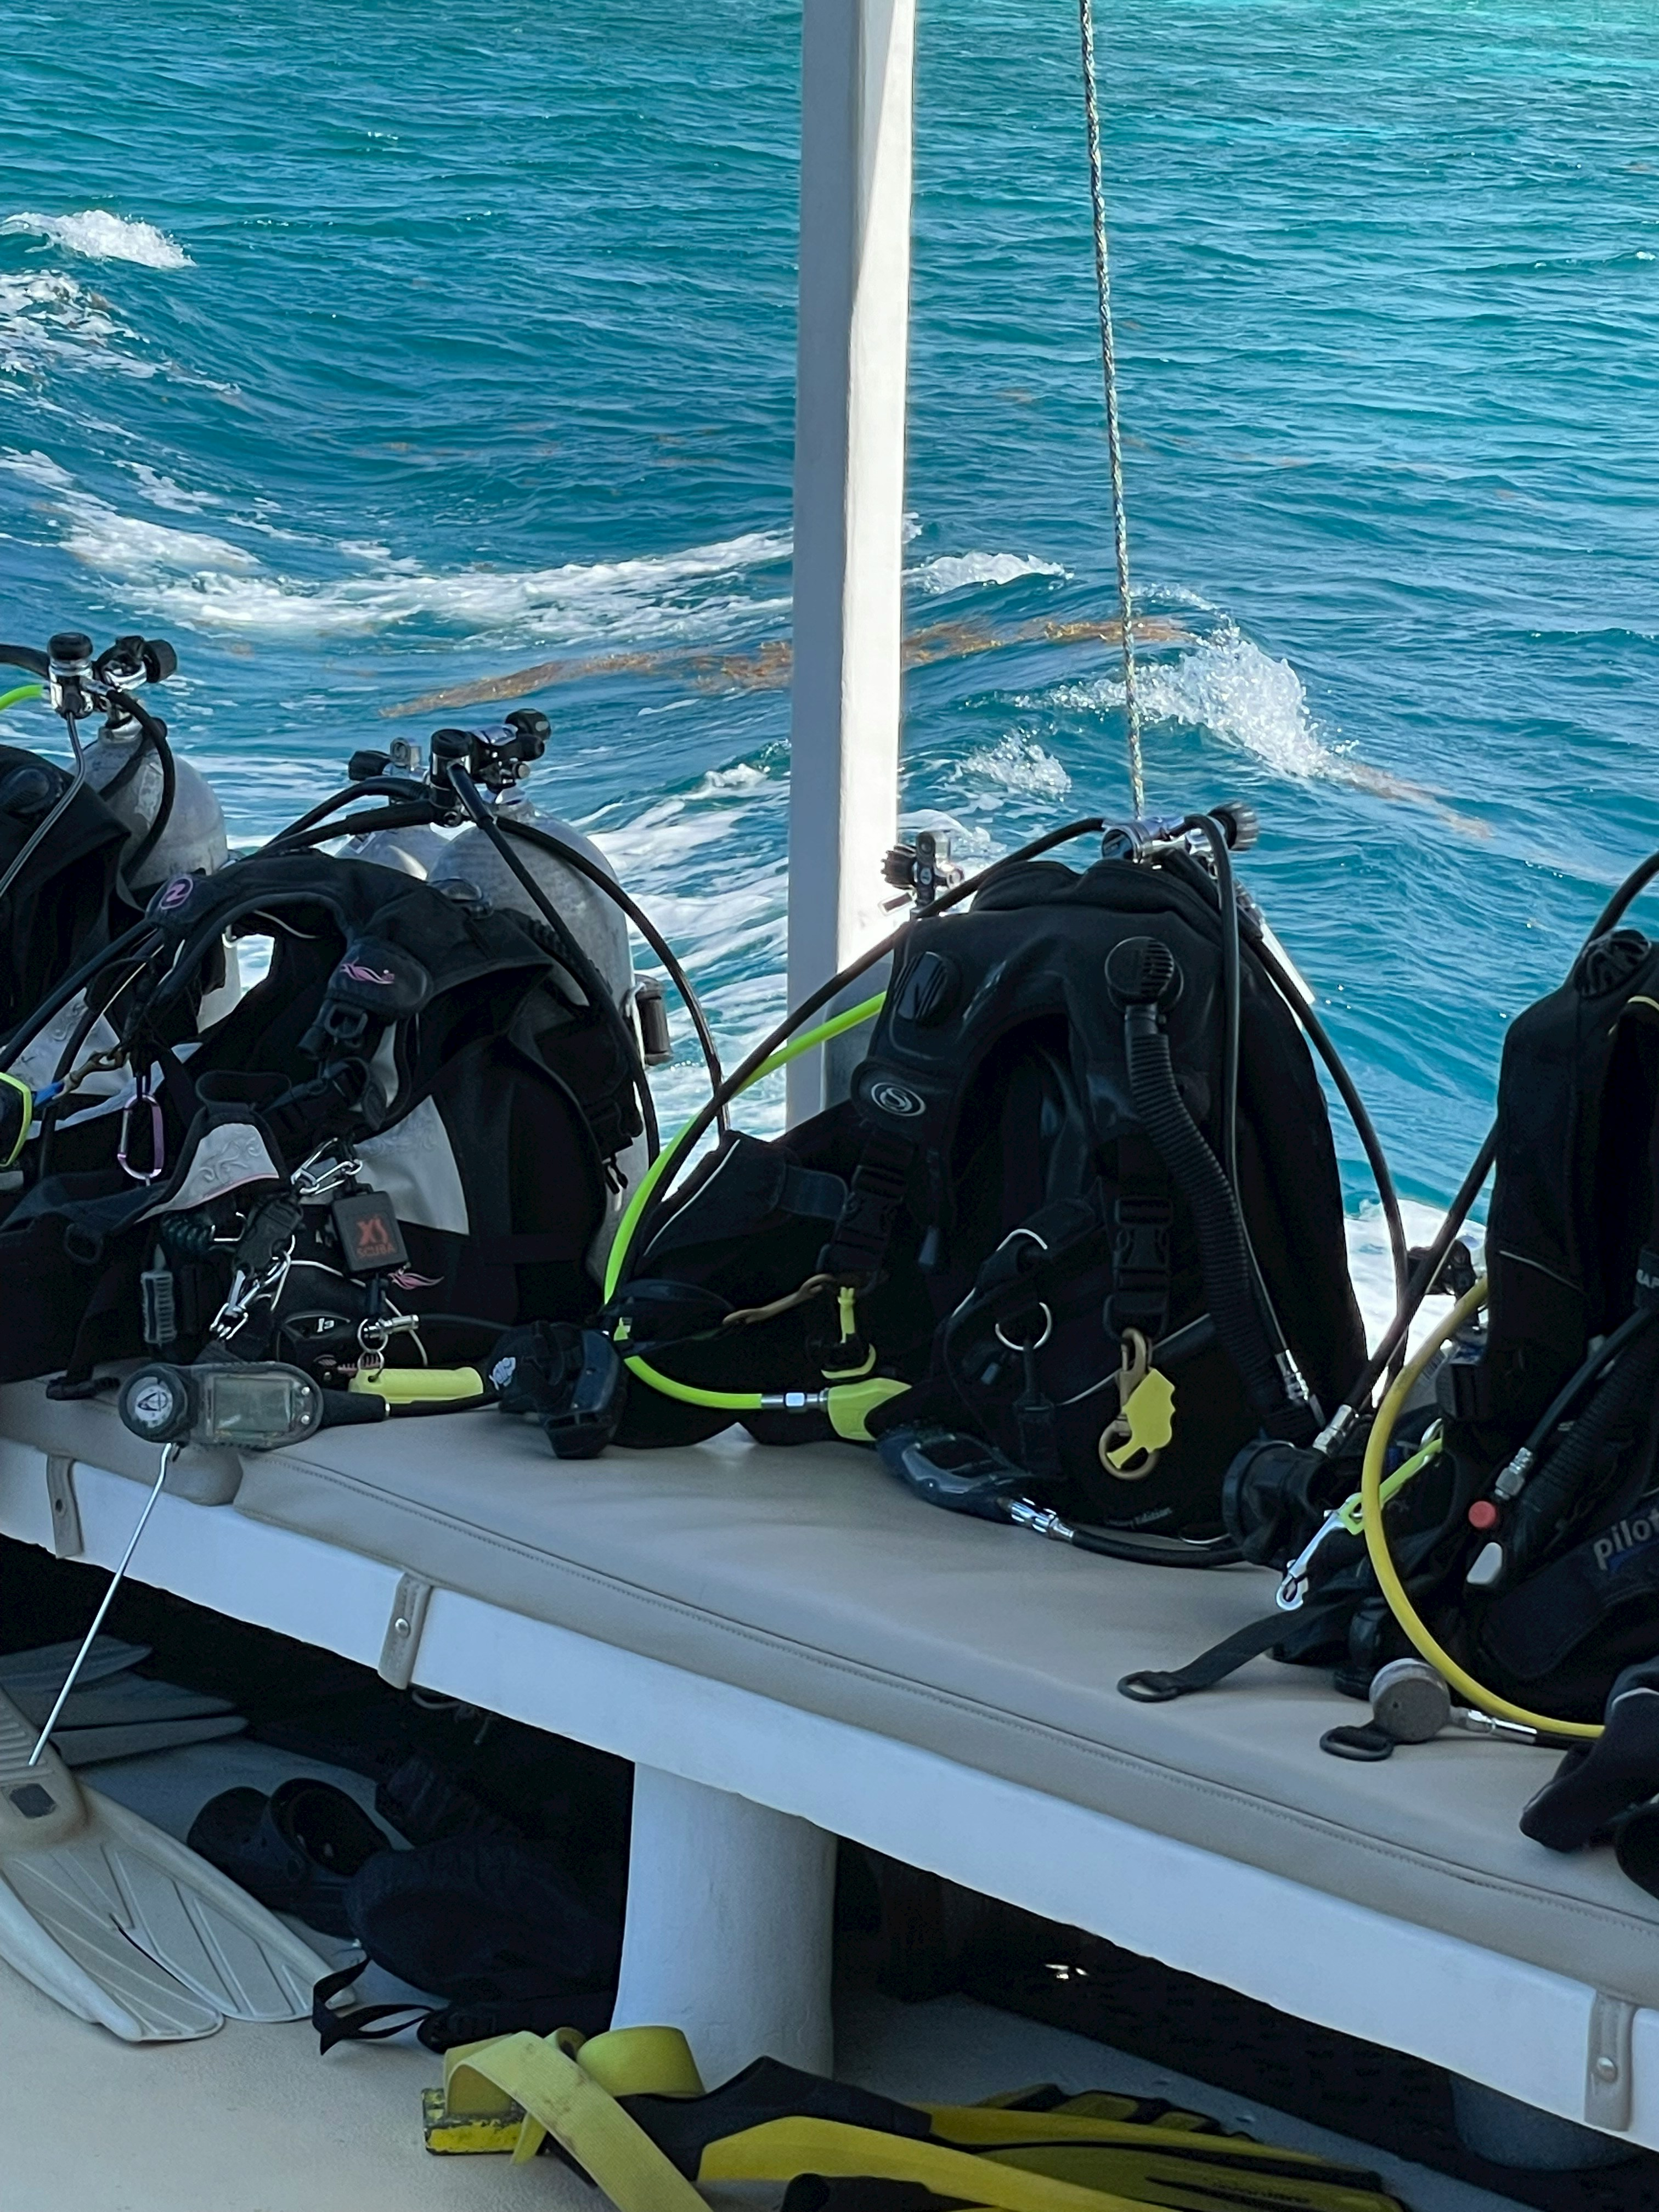
\includegraphics[height=3cm]{blocs}\hfill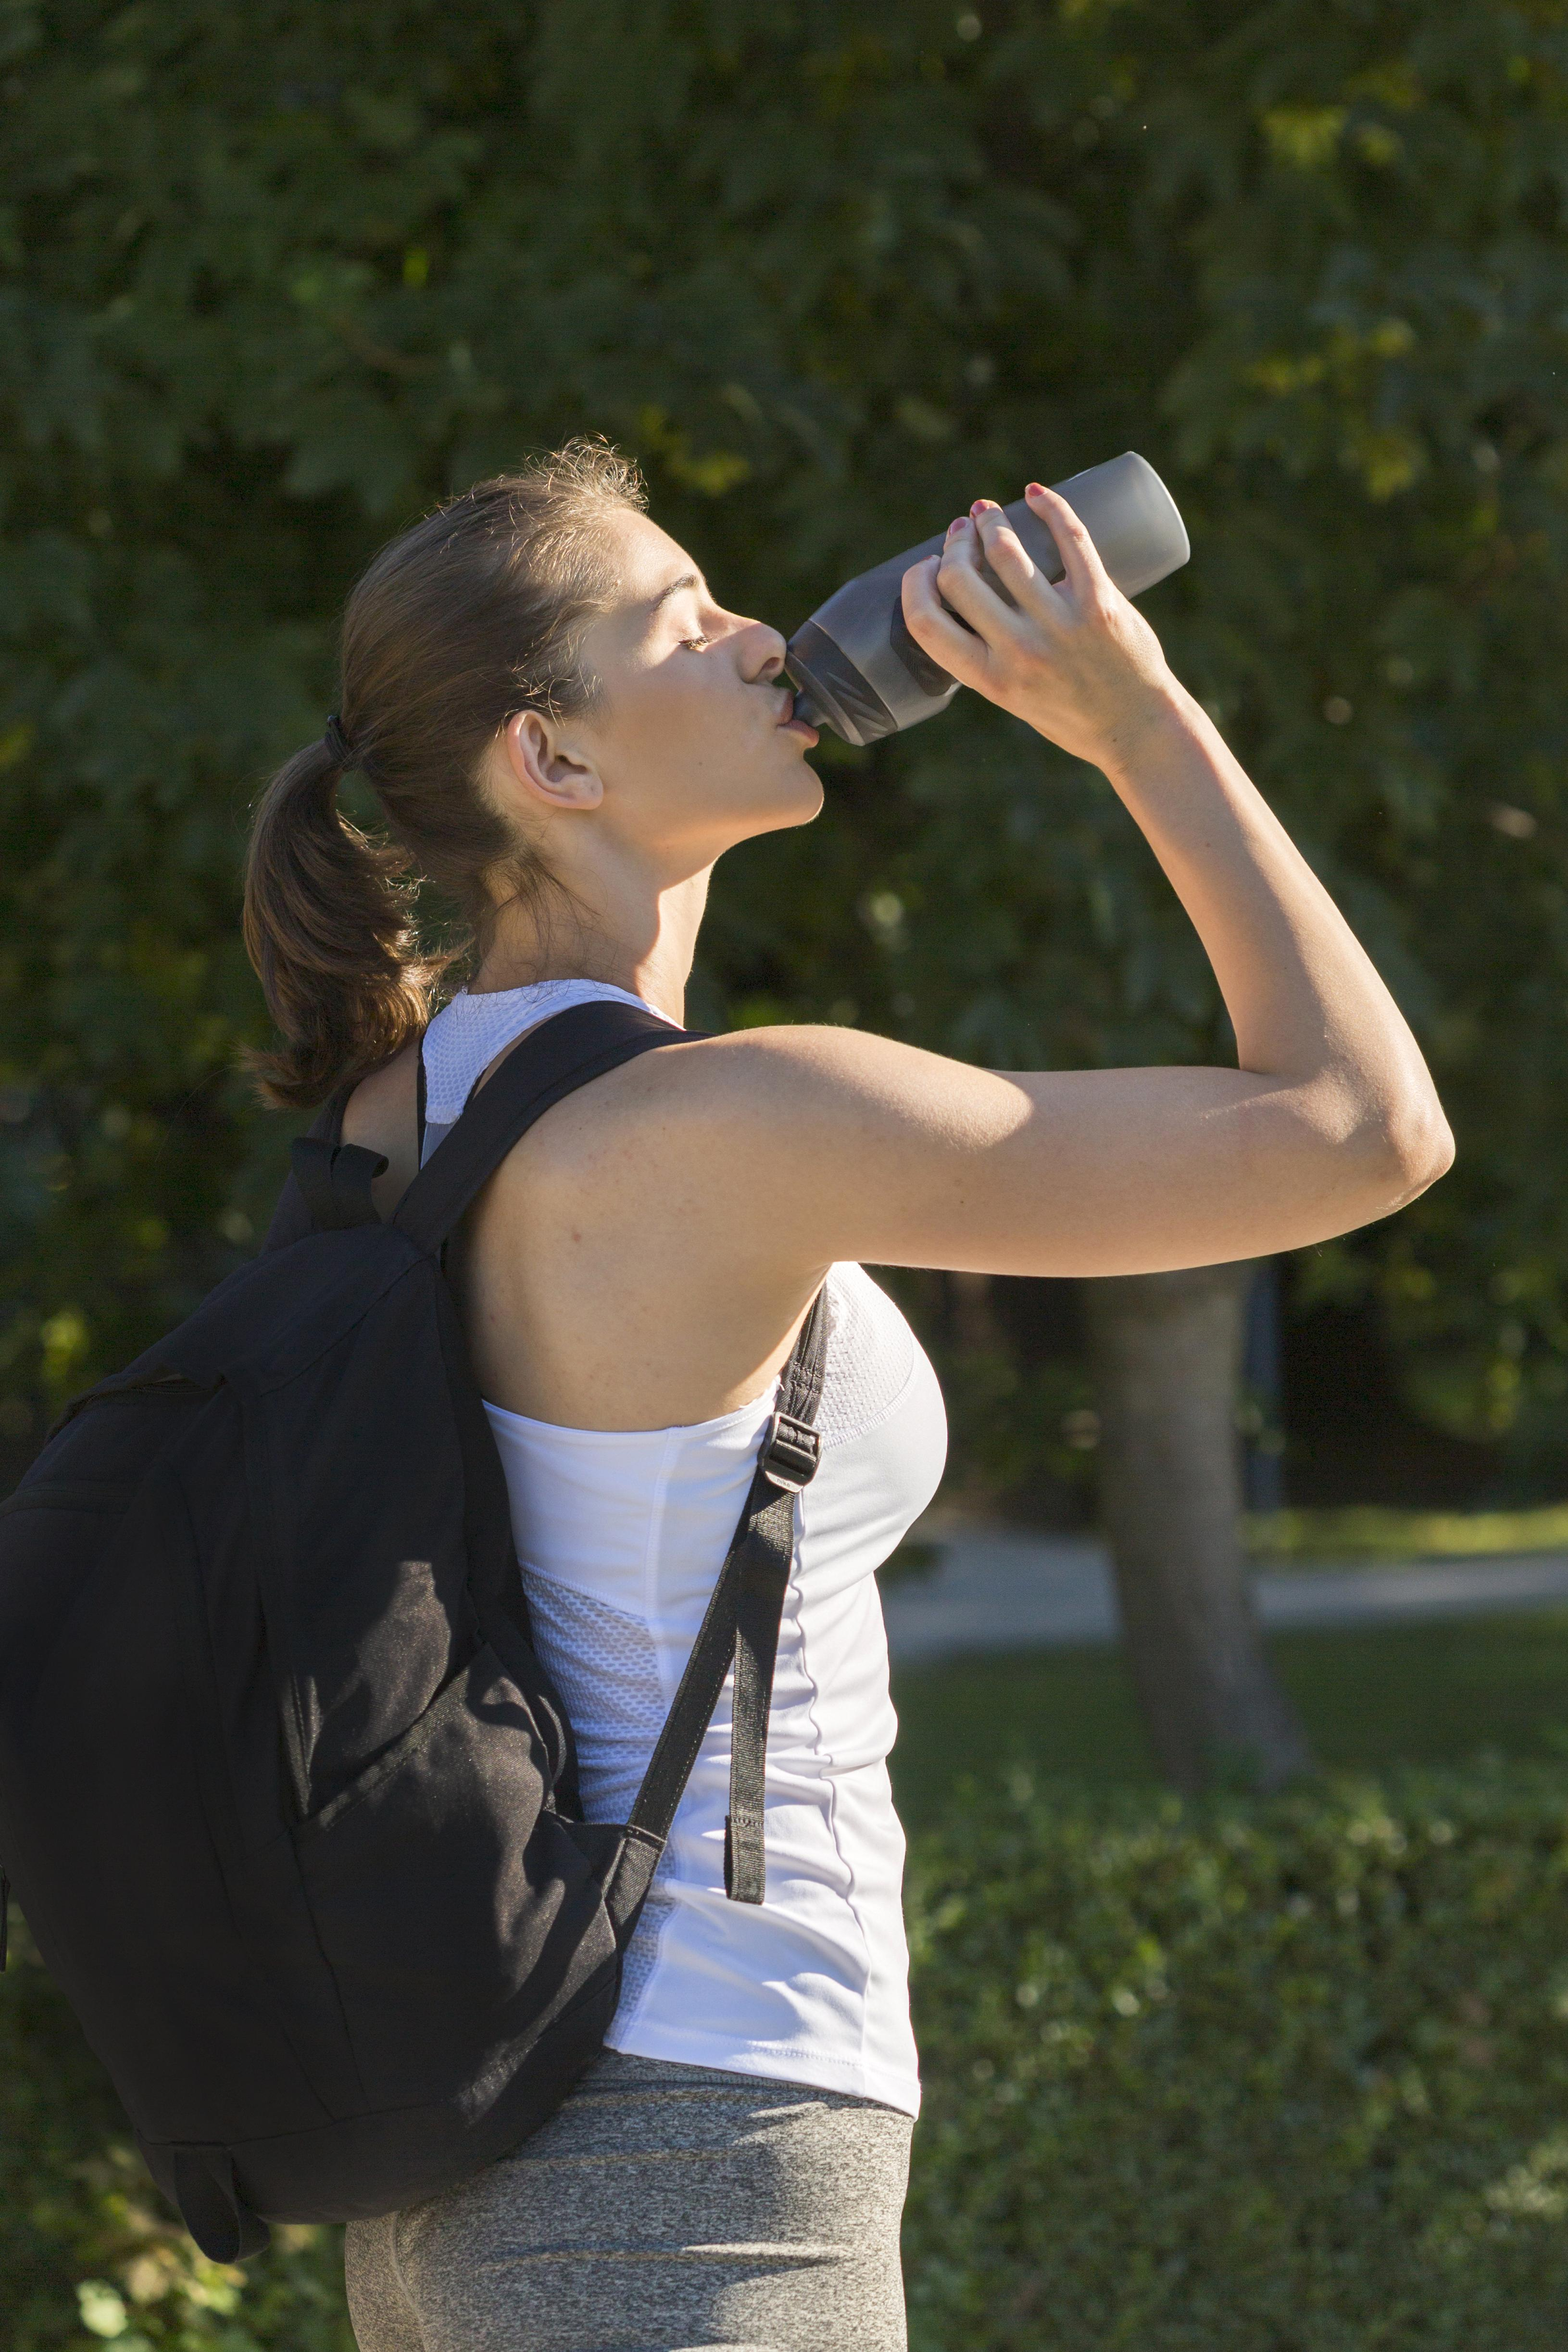
\includegraphics[height=3cm]{hydrate}\hfill\null%
\begin{block}{}
\begin{itemize}[<+->]
\item Déséquipe, matériel fixé, rien ne traîne;
\item on se sèche;
\item on s'hydrate.
\end{itemize}
\end{block}
\end{frame}

\begin{frame}{Après la plongée}
\begin{block}{}
\begin{itemize}
\item<1-> \twemoji{woman in lotus position: medium skin tone}Pas d'efforts;
\item<.-> pas d'apnée;
\item<.-> pas d'altitude (montagne, avion);
\item<2-> on continue de s'hydrater;
\item<3-> on rince si possible le matériel;
\item<3-> on complète son carnet de plongée;
\item<3-> on range;
\item<4> on rentre;
\item<4> on rince le matériel si non rincé, on l'étend;
\item<4> on est heureux(se).
\end{itemize}
\end{block}
\makebox[0pt][l]{\raisebox{4.5cm}[0pt][0pt]{\rule{0.6\textwidth}{0pt}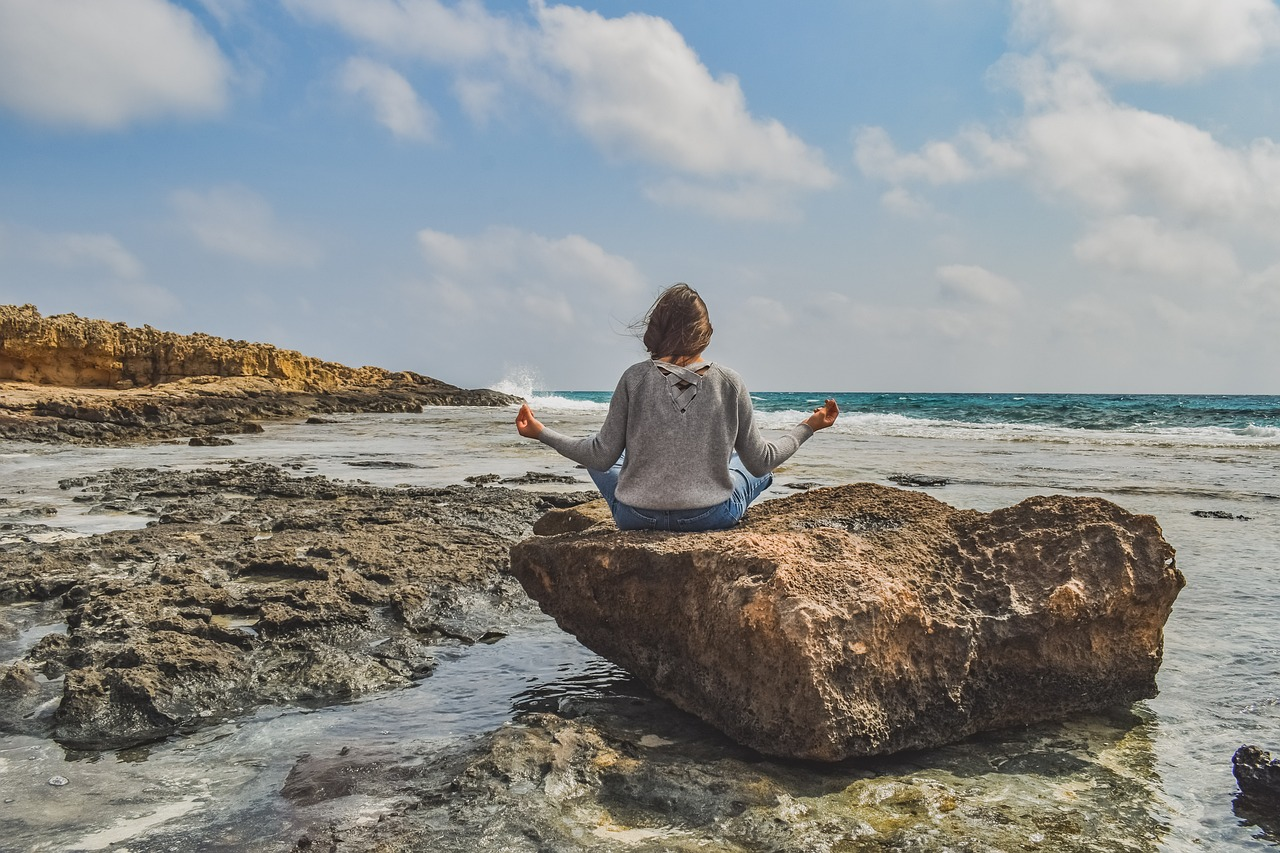
\includegraphics[width=3cm]{zen}}}%
\only<2->{\makebox[0pt][l]{\raisebox{1cm}[0pt][0pt]{\rule{0.72\textwidth}{0pt}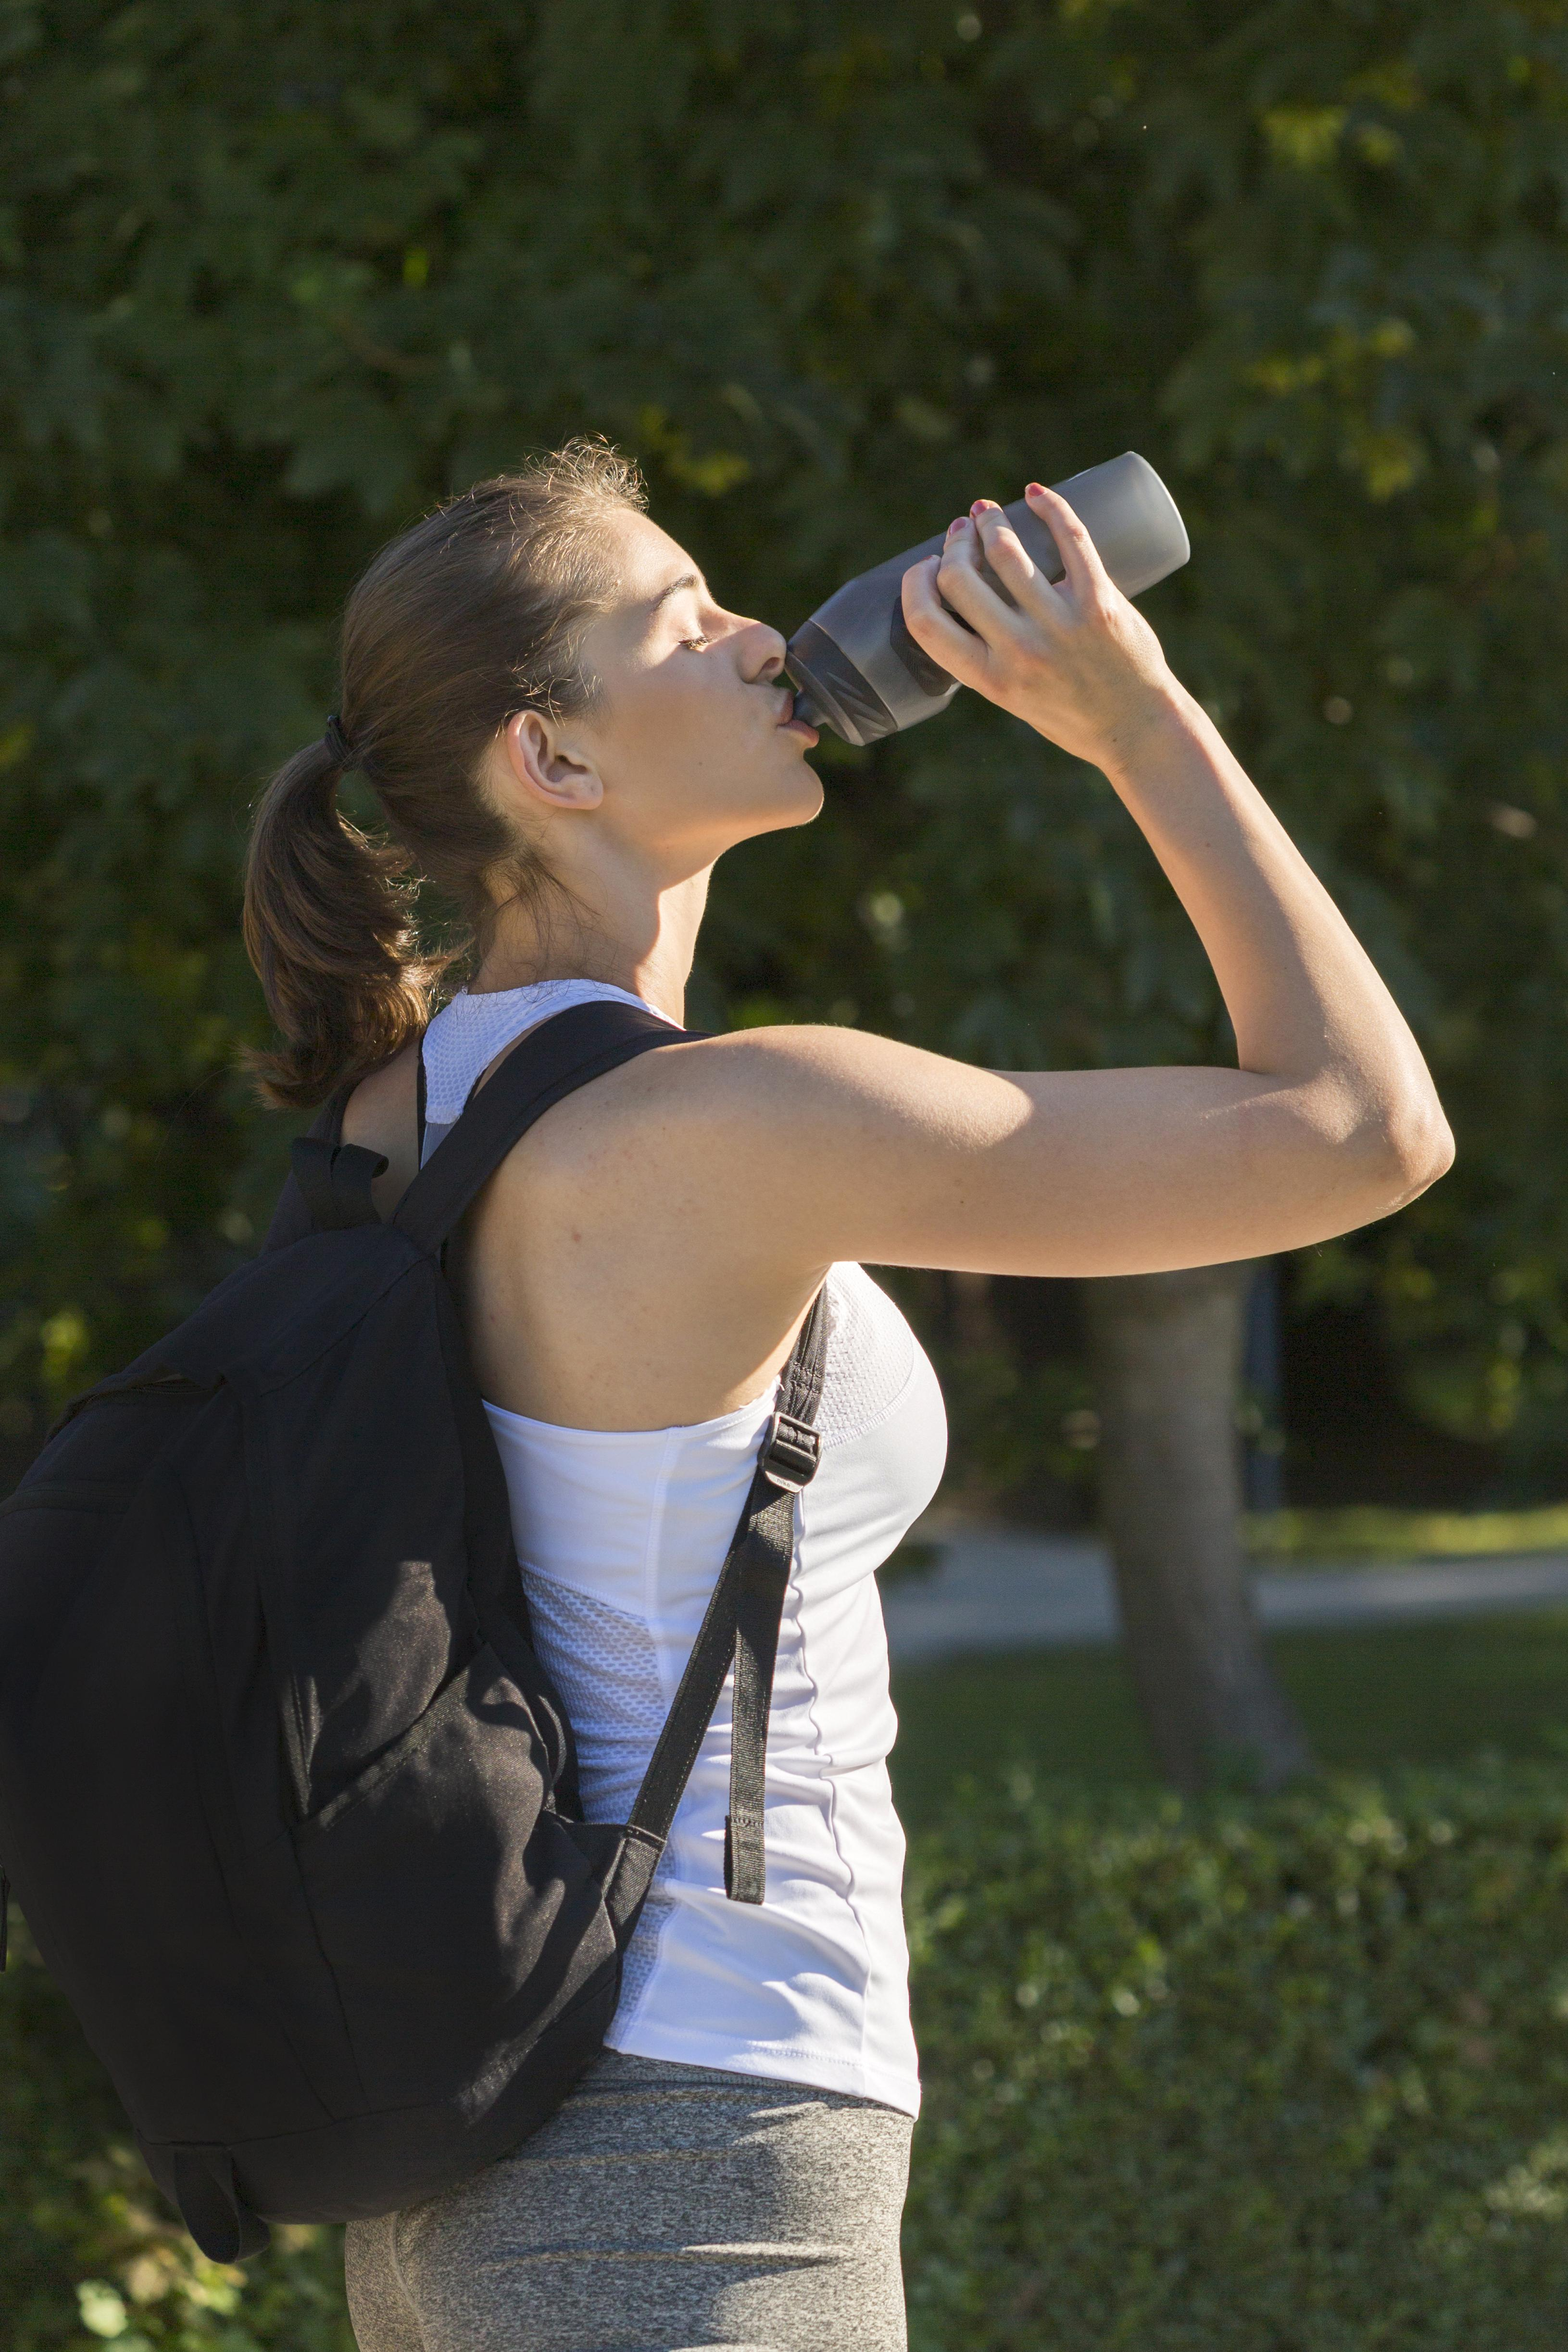
\includegraphics[width=2.7cm]{hydrate}}}}%
\only<3->{\makebox[0pt][l]{\raisebox{2cm}[0pt][0pt]{\rule{0.62\textwidth}{0pt}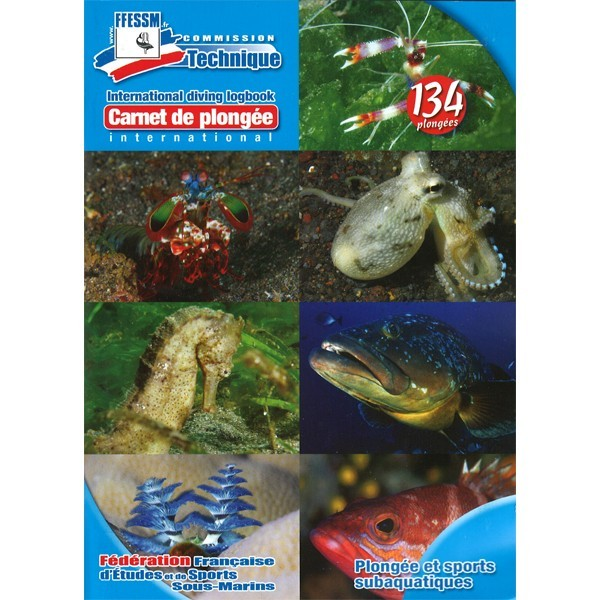
\includegraphics[width=2.5cm]{carnet_plongee}}}}%
\only<4>{\makebox[0pt][l]{\raisebox{2.1cm}[0pt][0pt]{\rule{0.61\textwidth}{0pt}\includegraphics[width=4cm]{bonheur}\makebox[0pt][r]{\tiny\textcolor{violet}{Image de Freepik}}}}}%
\end{frame}

\subsection{À l'AMP}
\begin{frame}{Les plongées \emph{techniques} pour le N1}
\begin{block}<only@1>{Ce qu'il faut viser}
\begin{itemize}
\item[\twemoji{penguin}] 4 plongées, limite\dots
\item[\twemoji{octopus}] 5 plongées, c'est mieux, 
\item[\twemoji{dolphin}] $\ge 6$ plongée, c'est cool.
%\item \twemoji{whale}, \twemoji{octopus}, \twemoji{fish}, \twemoji{tropical_fish}, \twemoji{blowfish}, \twemoji{penguin}, \twemoji{dolphin}, \twemoji{spouting whale}
\end{itemize}
\end{block}
\only<2>{%
\framesubtitle{Méjean}
\begin{minipage}{0.48\textwidth}
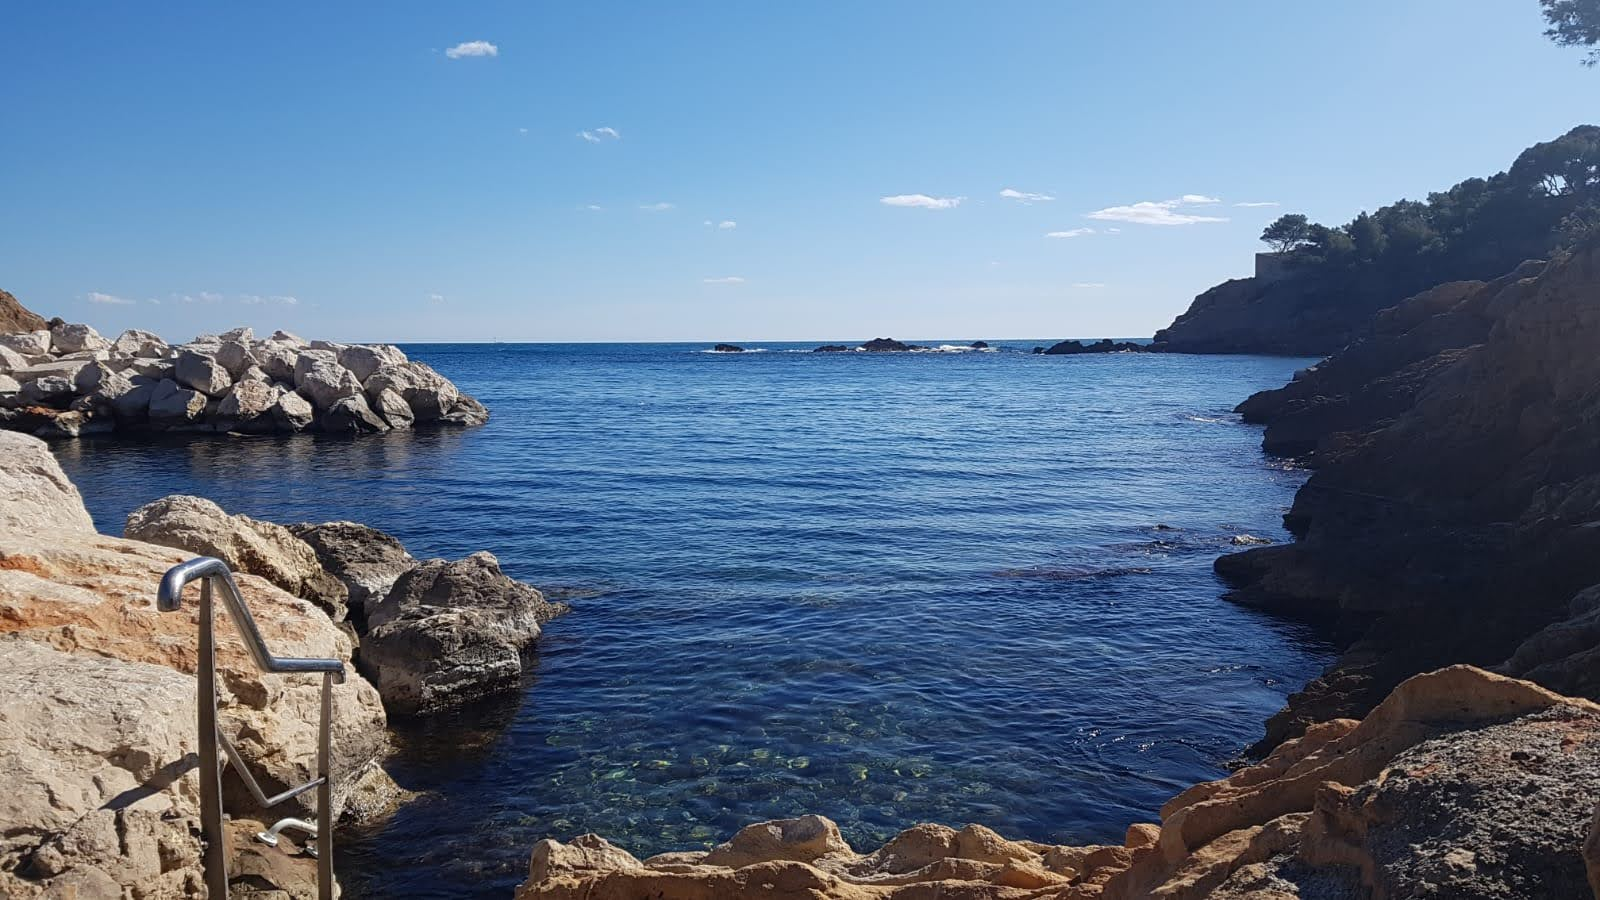
\includegraphics[width=\textwidth]{Mejean}
\end{minipage}\hfill
\begin{minipage}{0.48\textwidth}
\begin{exampleblock}{Idéal pour la mise à l'eau}
\begin{itemize}
\item départ du bord
\item protégé
\item peu profond
\end{itemize}
\end{exampleblock}
\end{minipage}
}%
\only<3>{%
\framesubtitle{Marseille}
\begin{minipage}{0.48\textwidth}
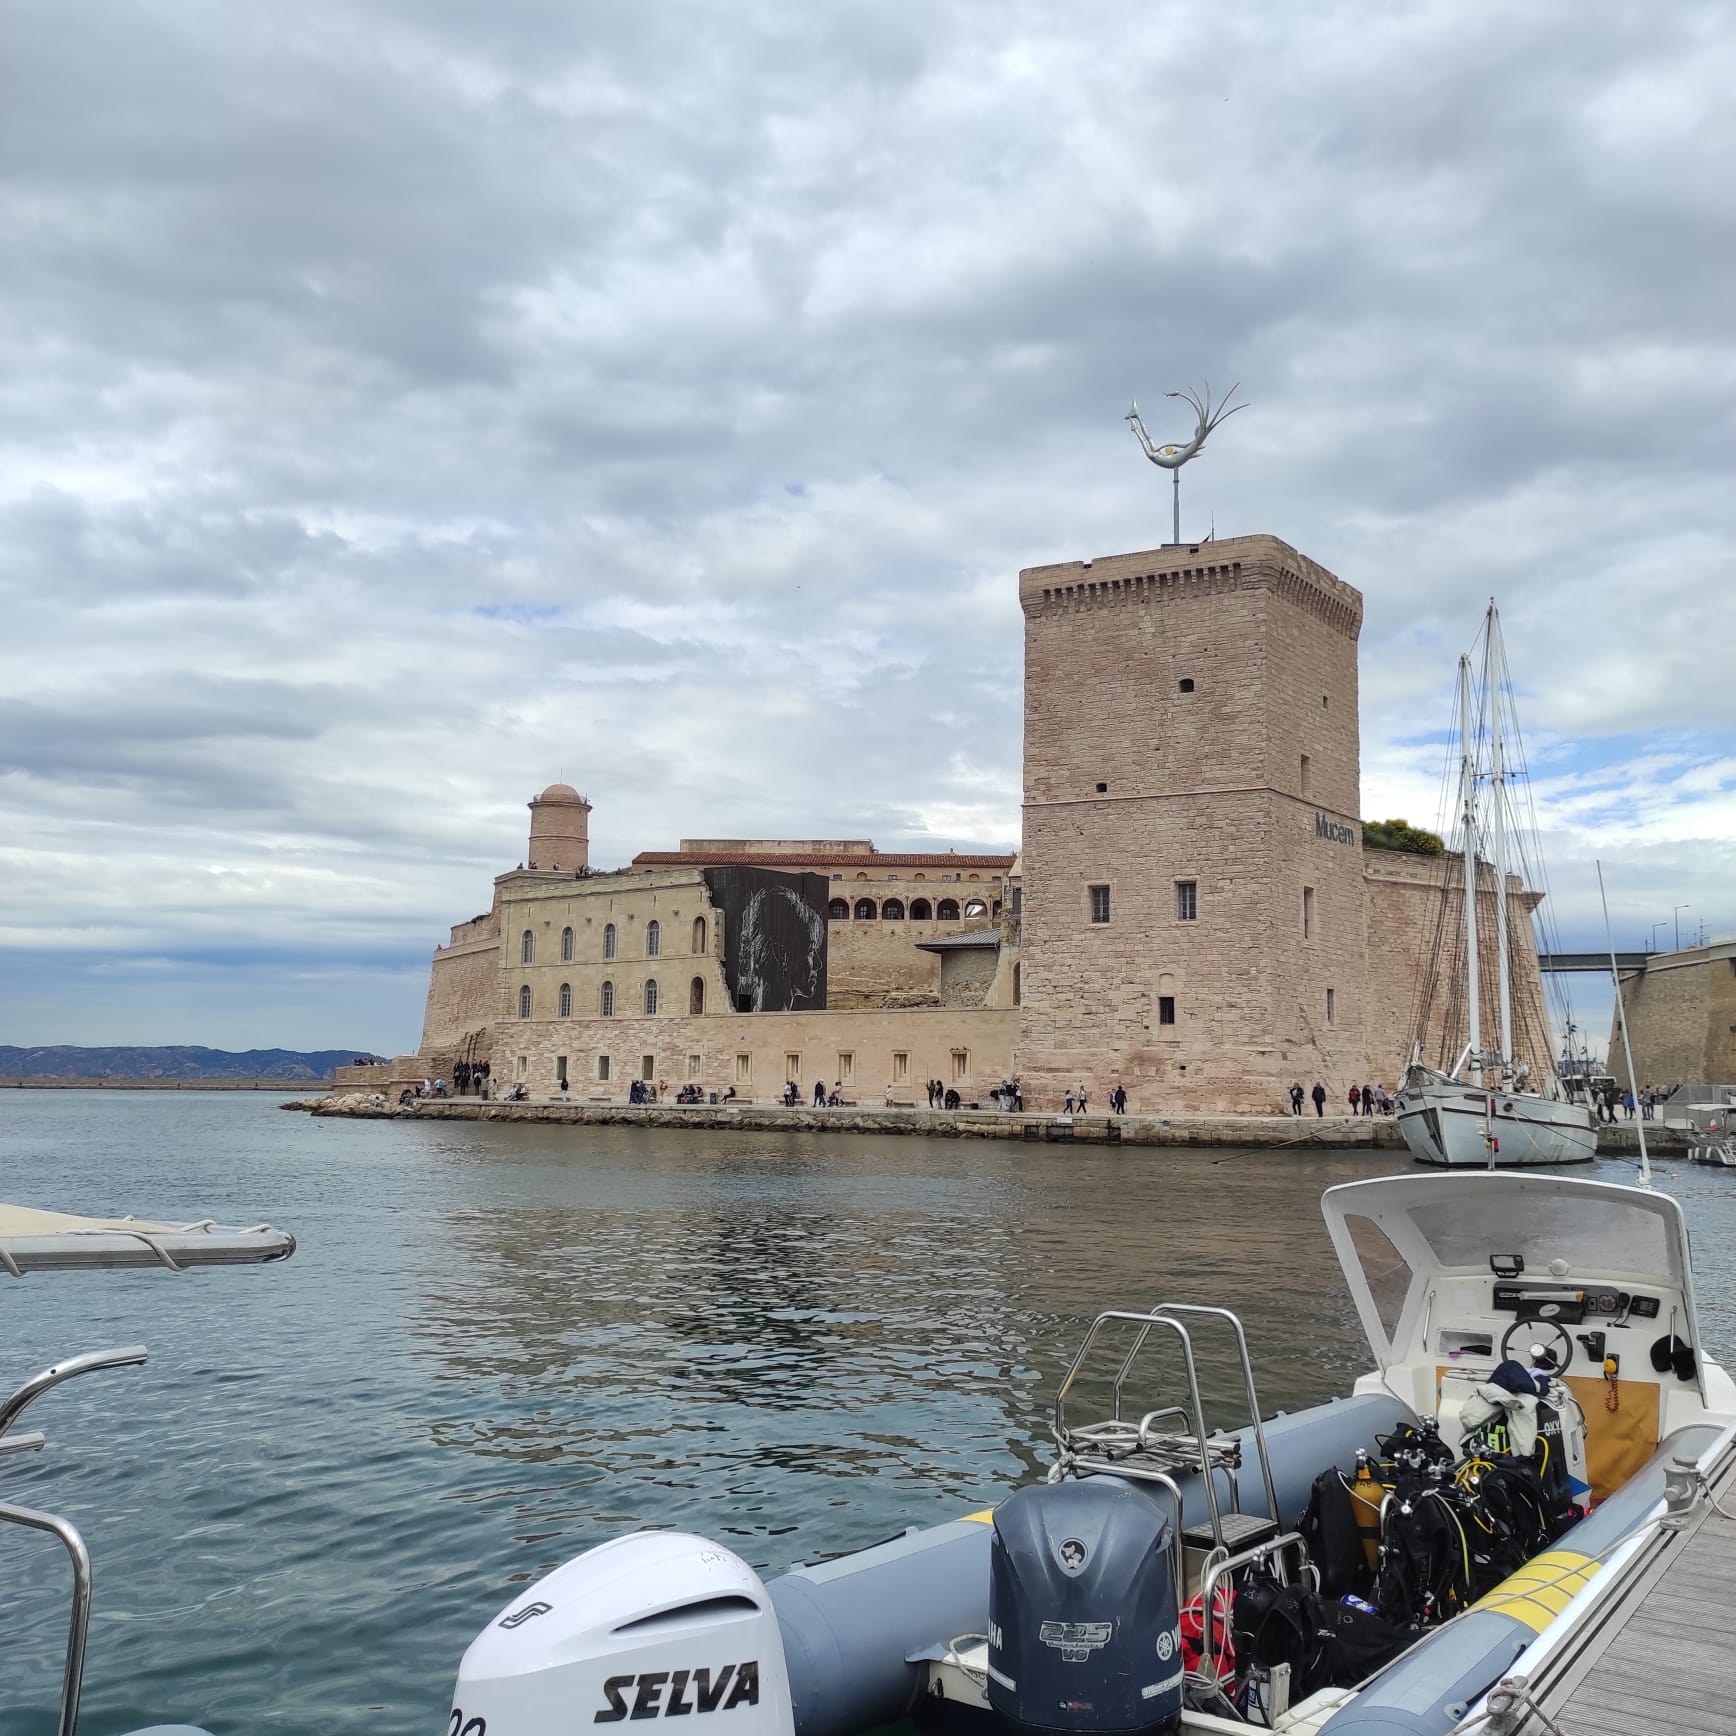
\includegraphics[width=\textwidth]{Marseille}
\end{minipage}\hfill
\begin{minipage}{0.48\textwidth}
\begin{exampleblock}{Idéal pour la suite}
\begin{itemize}
\item bonne visibilité
\item bascule arrière facile
\end{itemize}
\end{exampleblock}
\end{minipage}
}%
\begin{alertblock}<only@4>{Et donc\dots}
\Large Favoriser un maximum ces sorties pour valider le N1!
\end{alertblock}%
\only<4>{%
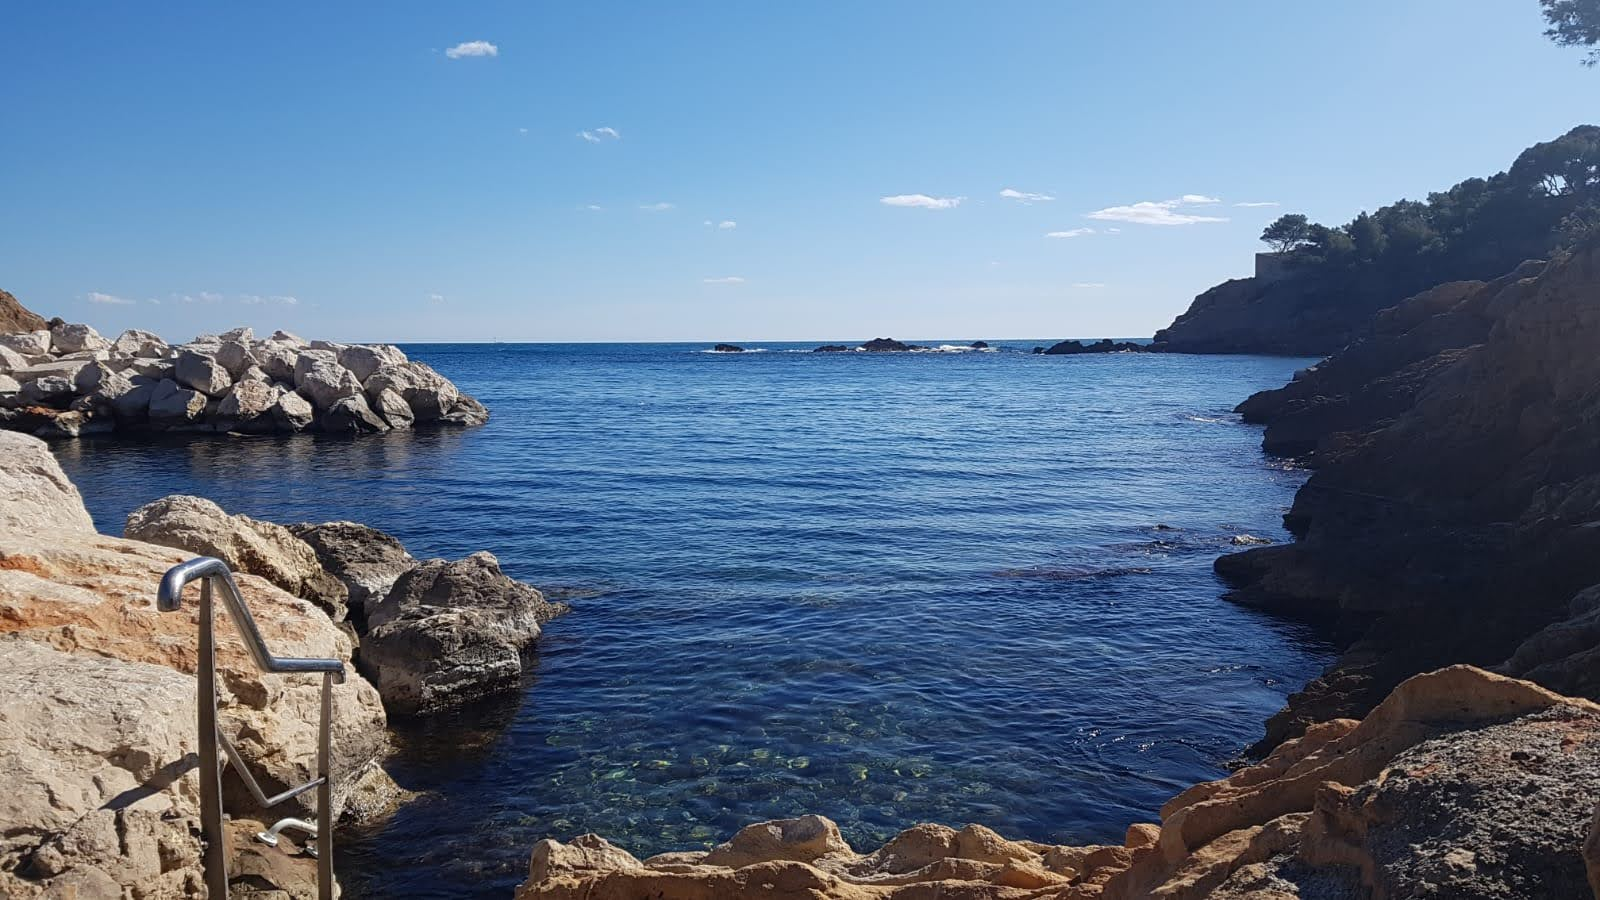
\includegraphics[width=0.48\textwidth]{Mejean}\hfill%
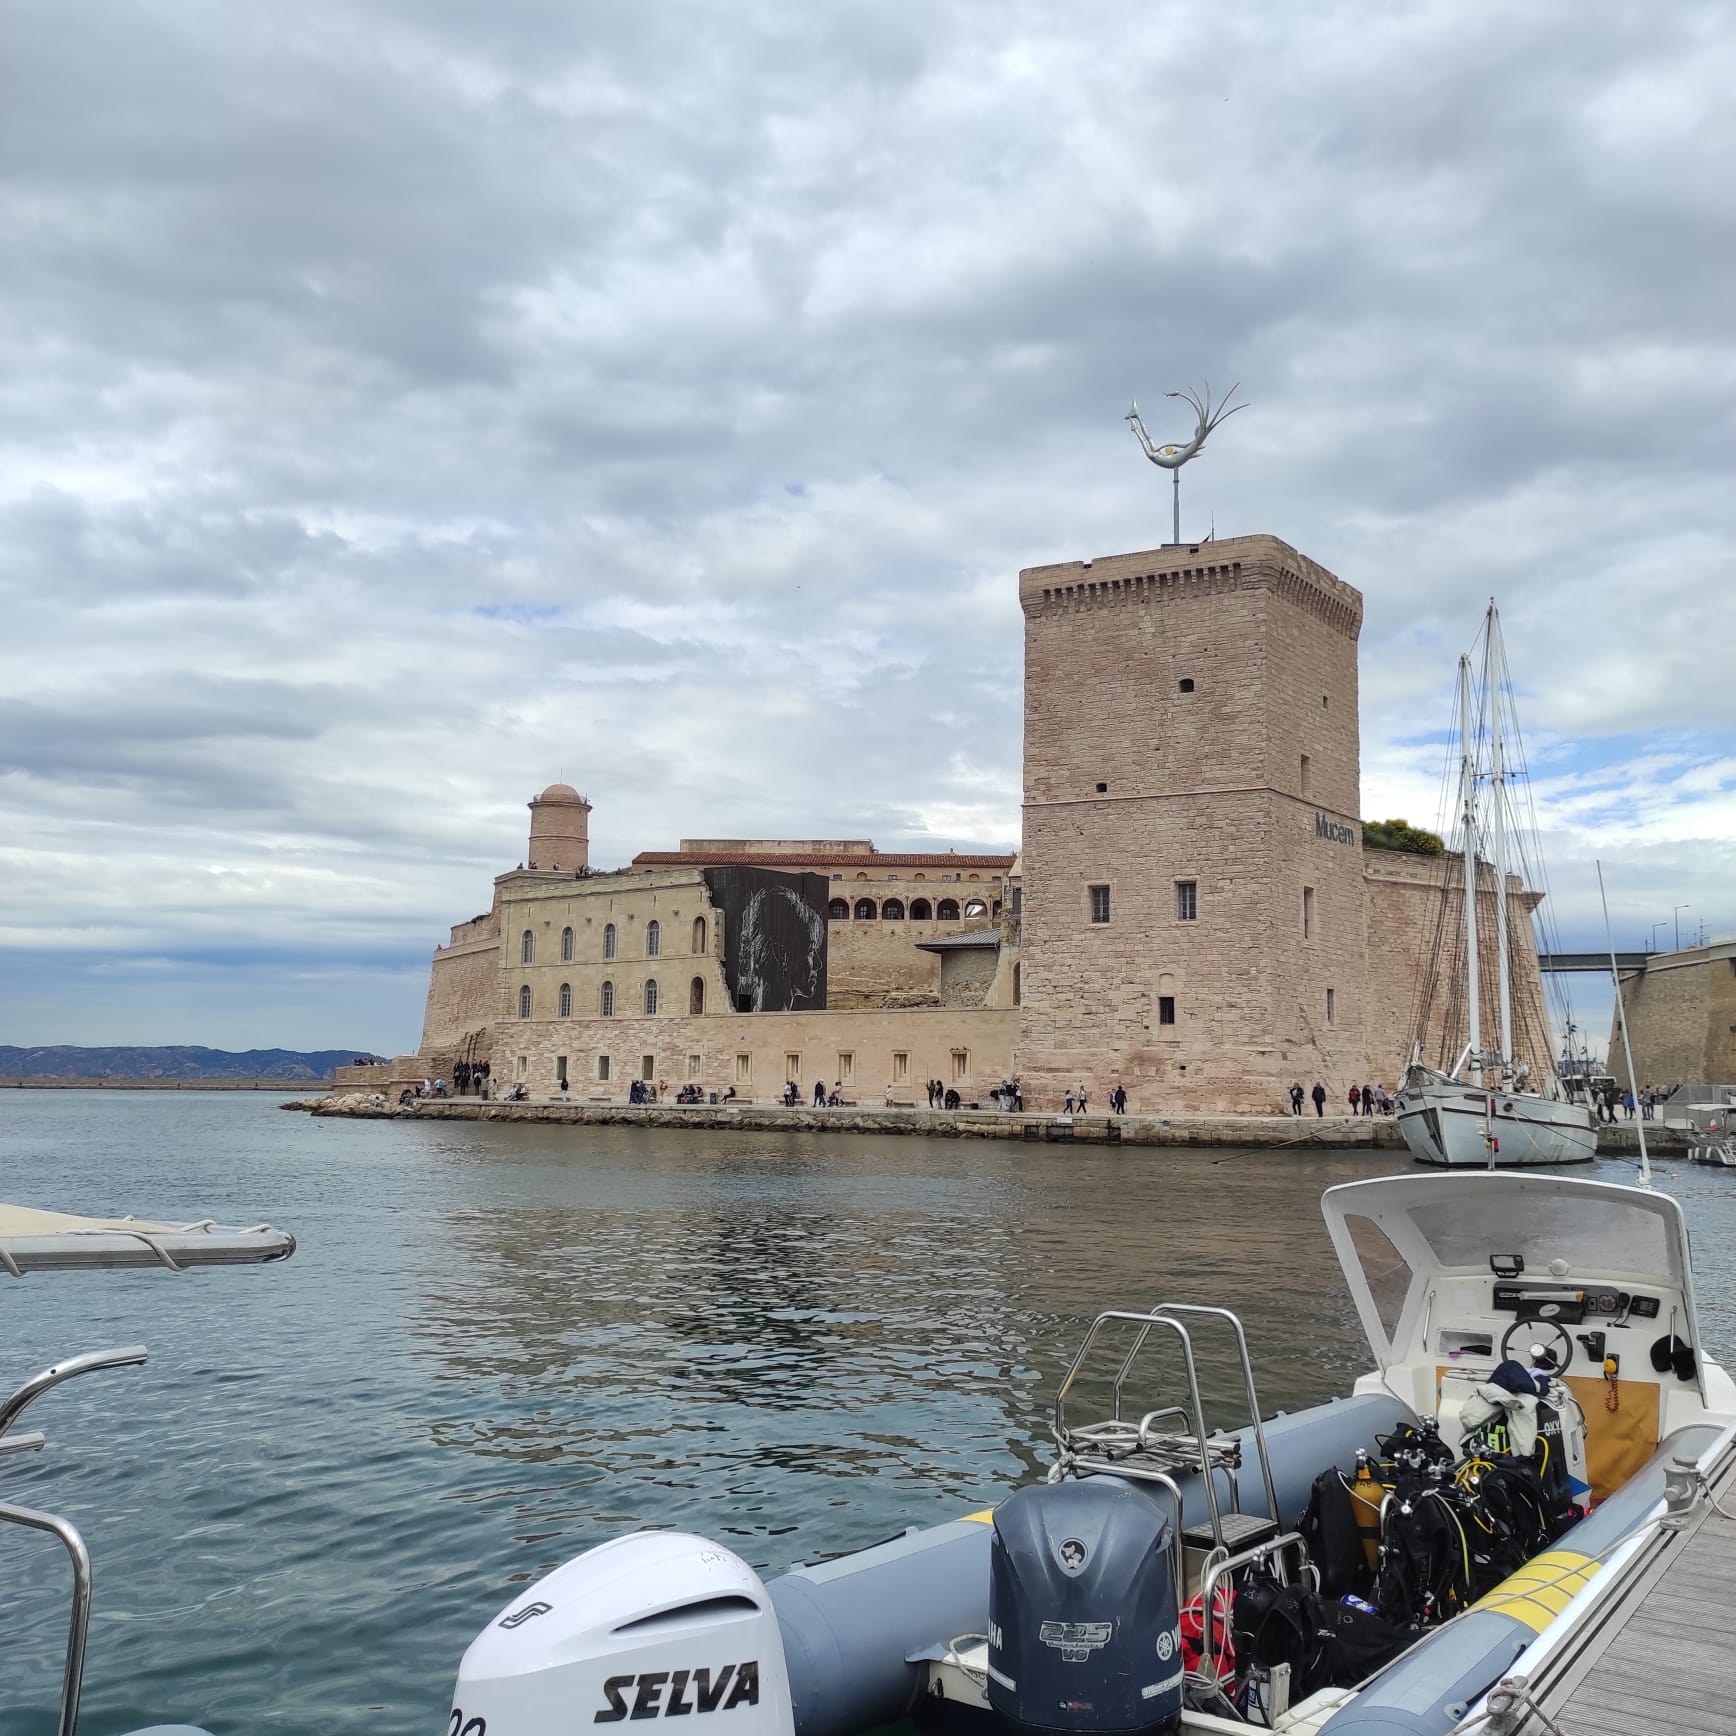
\includegraphics[width=0.4\textwidth]{Marseille}%
}%
%
\begin{alertblock}<only@5>{Date limite}
\parshape 3
0.16\textwidth 0.84\textwidth
0.16\textwidth 0.84\textwidth
0pt \textwidth
\squash{\rule{0pt}{1.5cm}\warningsign}%
\huge Remise des diplômes le \datelimite\ $\Rightarrow$
\tracingifs=2
faire ses plongées techniques \EMPH{au plus tard}
à cette sortie
\end{alertblock}%
\end{frame}

\begin{frame}{Inscription}
\begin{block}{}
\begin{center}
S'inscrire à une sortie
\end{center}
\end{block}
\end{frame}

\includepdf[pages=-]{AMP-Participer_aux_evenements_juin_2025}



\section{Respect de l'environnement}
\begin{frame}{Un palmage efficace et respectueux}
\begin{alertblock}{}
\danger{\Large Le milieu sous-marin est fragile! Il se respecte.}
\end{alertblock}

\begin{itemize}[<+(1)->]
\item Plongée \EMPH{loisir} $=$ observation de la beauté sous-marine
\item[$\Rightarrow$] minimum de mouvements/perturbations:
  \begin{itemize}[<+->]
    \item stabilisé(e): palme ni contre le fond ni en haut;
    \item calme, attention aux alentours;
    \item matériel bien rangé: mano, octopus, \dots\ $\Rightarrow$ ne râclent pas le fond;
    \item pas toucher! Ça abîme et c'est dangereux;
    \item[$\Rightarrow$] on s'économise et on ne vandalise rien.
  \end{itemize}
\end{itemize}
\end{frame}

\begin{frame}{La charte internationale du plongeur responsable}
{\url{https://www.longitude181.org/la-charte/}}
\centering\includefullheightgraphics{charte}
\end{frame}


\begin{frame}{Méjean}
\centering%
\photo<1>{Mejean}{\textwidth}
\photo<2>[Codium en boule]{Codium}{\textwidth}
\photo<3>[An{\'e}mone verte]{anemone}{\textwidth}
\photo<4>[Ascidie coloniale]{ascidie}{\textwidth}
\photo<5>[Bernard\ l'hermite]{bernard}{\textwidth}
\photo<6>[{\'E}toile\ de\ mer\ peigne]{etoile_peigne}{\textwidth}
\photo<7>[Gobie\ {\`a}\ t{\^e}te\ jaune]{gobie}{0.6\textwidth}
\photo<7>[Gobie\ svelte]{gobie_svelte}{0.3\textwidth}
\photo<8>[Cr{\'e}nilabre\ cendr{\'e}]{crenilabre}{\textwidth}
\photo<9>[Holothurie]{holothurie}{\textwidth}
\photo<10>[Oursin\ violet]{oursin}{\textwidth}
\photo<11>[Test\ d'oursin\ violet]{test_oursin}{\textwidth}
\photo<12>[Sabelle]{sabelle}{0.35\textwidth}
\photo<13>[Seiche]{seiche}{\textwidth}
\photo<14>[Thuridille de Hope]{thuridille}{\textwidth}
\photo<15>[Plein de choses]{scene}{\textwidth}
\photo<16>[Des\ grosses\ b{\^e}tes]{plongeursAMP}{0.8\textwidth}
\end{frame}


\setbeamertemplate{background}{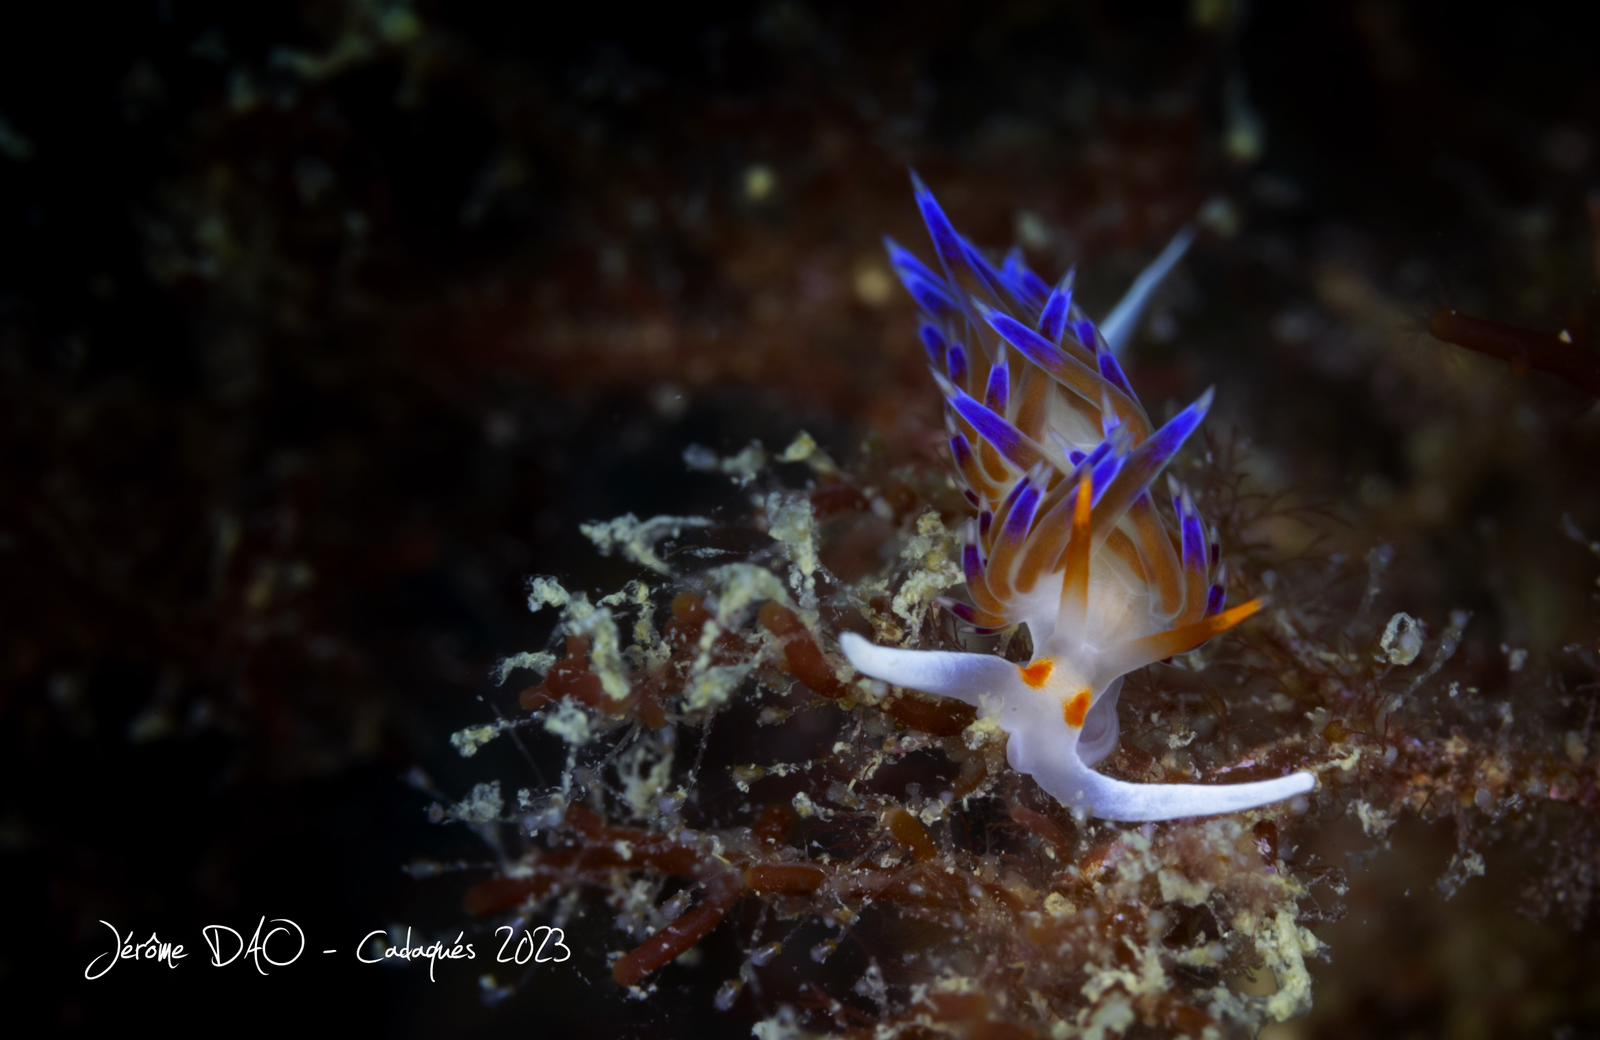
\includegraphics[height=\paperheight]{Cadaques-2023}}
\begin{frame}{Merci de votre attention!}
\color{white}
Cours N1 en ligne de la fédération:\\\url{https://formation.ffessm.fr/cours/cours-sequence/plonger-avec-la-ffessm-niveau-1}
\begin{center}
\Huge Des questions?
\end{center}
\end{frame}

\end{document}
